\documentclass[11pt]{article}

    \usepackage[breakable]{tcolorbox}
    \usepackage{parskip} % Stop auto-indenting (to mimic markdown behaviour)
    

    % Basic figure setup, for now with no caption control since it's done
    % automatically by Pandoc (which extracts ![](path) syntax from Markdown).
    \usepackage{graphicx}
    % Maintain compatibility with old templates. Remove in nbconvert 6.0
    \let\Oldincludegraphics\includegraphics
    % Ensure that by default, figures have no caption (until we provide a
    % proper Figure object with a Caption API and a way to capture that
    % in the conversion process - todo).
    \usepackage{caption}
    \DeclareCaptionFormat{nocaption}{}
    \captionsetup{format=nocaption,aboveskip=0pt,belowskip=0pt}

    \usepackage{float}
    \floatplacement{figure}{H} % forces figures to be placed at the correct location
    \usepackage{xcolor} % Allow colors to be defined
    \usepackage{enumerate} % Needed for markdown enumerations to work
    \usepackage{geometry} % Used to adjust the document margins
    \usepackage{amsmath} % Equations
    \usepackage{amssymb} % Equations
    \usepackage{textcomp} % defines textquotesingle
    % Hack from http://tex.stackexchange.com/a/47451/13684:
    \AtBeginDocument{%
        \def\PYZsq{\textquotesingle}% Upright quotes in Pygmentized code
    }
    \usepackage{upquote} % Upright quotes for verbatim code
    \usepackage{eurosym} % defines \euro

    \usepackage{iftex}
    \ifPDFTeX
        \usepackage[T1]{fontenc}
        \IfFileExists{alphabeta.sty}{
              \usepackage{alphabeta}
          }{
              \usepackage[mathletters]{ucs}
              \usepackage[utf8x]{inputenc}
          }
    \else
        \usepackage{fontspec}
        \usepackage{unicode-math}
    \fi

    \usepackage{fancyvrb} % verbatim replacement that allows latex
    \usepackage{grffile} % extends the file name processing of package graphics
                         % to support a larger range
    \makeatletter % fix for old versions of grffile with XeLaTeX
    \@ifpackagelater{grffile}{2019/11/01}
    {
      % Do nothing on new versions
    }
    {
      \def\Gread@@xetex#1{%
        \IfFileExists{"\Gin@base".bb}%
        {\Gread@eps{\Gin@base.bb}}%
        {\Gread@@xetex@aux#1}%
      }
    }
    \makeatother
    \usepackage[Export]{adjustbox} % Used to constrain images to a maximum size
    \adjustboxset{max size={0.9\linewidth}{0.9\paperheight}}

    % The hyperref package gives us a pdf with properly built
    % internal navigation ('pdf bookmarks' for the table of contents,
    % internal cross-reference links, web links for URLs, etc.)
    \usepackage{hyperref}
    % The default LaTeX title has an obnoxious amount of whitespace. By default,
    % titling removes some of it. It also provides customization options.
    \usepackage{titling}
    \usepackage{longtable} % longtable support required by pandoc >1.10
    \usepackage{booktabs}  % table support for pandoc > 1.12.2
    \usepackage{array}     % table support for pandoc >= 2.11.3
    \usepackage{calc}      % table minipage width calculation for pandoc >= 2.11.1
    \usepackage[inline]{enumitem} % IRkernel/repr support (it uses the enumerate* environment)
    \usepackage[normalem]{ulem} % ulem is needed to support strikethroughs (\sout)
                                % normalem makes italics be italics, not underlines
    \usepackage{soul}      % strikethrough (\st) support for pandoc >= 3.0.0
    \usepackage{mathrsfs}
    

    
    % Colors for the hyperref package
    \definecolor{urlcolor}{rgb}{0,.145,.698}
    \definecolor{linkcolor}{rgb}{.71,0.21,0.01}
    \definecolor{citecolor}{rgb}{.12,.54,.11}

    % ANSI colors
    \definecolor{ansi-black}{HTML}{3E424D}
    \definecolor{ansi-black-intense}{HTML}{282C36}
    \definecolor{ansi-red}{HTML}{E75C58}
    \definecolor{ansi-red-intense}{HTML}{B22B31}
    \definecolor{ansi-green}{HTML}{00A250}
    \definecolor{ansi-green-intense}{HTML}{007427}
    \definecolor{ansi-yellow}{HTML}{DDB62B}
    \definecolor{ansi-yellow-intense}{HTML}{B27D12}
    \definecolor{ansi-blue}{HTML}{208FFB}
    \definecolor{ansi-blue-intense}{HTML}{0065CA}
    \definecolor{ansi-magenta}{HTML}{D160C4}
    \definecolor{ansi-magenta-intense}{HTML}{A03196}
    \definecolor{ansi-cyan}{HTML}{60C6C8}
    \definecolor{ansi-cyan-intense}{HTML}{258F8F}
    \definecolor{ansi-white}{HTML}{C5C1B4}
    \definecolor{ansi-white-intense}{HTML}{A1A6B2}
    \definecolor{ansi-default-inverse-fg}{HTML}{FFFFFF}
    \definecolor{ansi-default-inverse-bg}{HTML}{000000}

    % common color for the border for error outputs.
    \definecolor{outerrorbackground}{HTML}{FFDFDF}

    % commands and environments needed by pandoc snippets
    % extracted from the output of `pandoc -s`
    \providecommand{\tightlist}{%
      \setlength{\itemsep}{0pt}\setlength{\parskip}{0pt}}
    \DefineVerbatimEnvironment{Highlighting}{Verbatim}{commandchars=\\\{\}}
    % Add ',fontsize=\small' for more characters per line
    \newenvironment{Shaded}{}{}
    \newcommand{\KeywordTok}[1]{\textcolor[rgb]{0.00,0.44,0.13}{\textbf{{#1}}}}
    \newcommand{\DataTypeTok}[1]{\textcolor[rgb]{0.56,0.13,0.00}{{#1}}}
    \newcommand{\DecValTok}[1]{\textcolor[rgb]{0.25,0.63,0.44}{{#1}}}
    \newcommand{\BaseNTok}[1]{\textcolor[rgb]{0.25,0.63,0.44}{{#1}}}
    \newcommand{\FloatTok}[1]{\textcolor[rgb]{0.25,0.63,0.44}{{#1}}}
    \newcommand{\CharTok}[1]{\textcolor[rgb]{0.25,0.44,0.63}{{#1}}}
    \newcommand{\StringTok}[1]{\textcolor[rgb]{0.25,0.44,0.63}{{#1}}}
    \newcommand{\CommentTok}[1]{\textcolor[rgb]{0.38,0.63,0.69}{\textit{{#1}}}}
    \newcommand{\OtherTok}[1]{\textcolor[rgb]{0.00,0.44,0.13}{{#1}}}
    \newcommand{\AlertTok}[1]{\textcolor[rgb]{1.00,0.00,0.00}{\textbf{{#1}}}}
    \newcommand{\FunctionTok}[1]{\textcolor[rgb]{0.02,0.16,0.49}{{#1}}}
    \newcommand{\RegionMarkerTok}[1]{{#1}}
    \newcommand{\ErrorTok}[1]{\textcolor[rgb]{1.00,0.00,0.00}{\textbf{{#1}}}}
    \newcommand{\NormalTok}[1]{{#1}}

    % Additional commands for more recent versions of Pandoc
    \newcommand{\ConstantTok}[1]{\textcolor[rgb]{0.53,0.00,0.00}{{#1}}}
    \newcommand{\SpecialCharTok}[1]{\textcolor[rgb]{0.25,0.44,0.63}{{#1}}}
    \newcommand{\VerbatimStringTok}[1]{\textcolor[rgb]{0.25,0.44,0.63}{{#1}}}
    \newcommand{\SpecialStringTok}[1]{\textcolor[rgb]{0.73,0.40,0.53}{{#1}}}
    \newcommand{\ImportTok}[1]{{#1}}
    \newcommand{\DocumentationTok}[1]{\textcolor[rgb]{0.73,0.13,0.13}{\textit{{#1}}}}
    \newcommand{\AnnotationTok}[1]{\textcolor[rgb]{0.38,0.63,0.69}{\textbf{\textit{{#1}}}}}
    \newcommand{\CommentVarTok}[1]{\textcolor[rgb]{0.38,0.63,0.69}{\textbf{\textit{{#1}}}}}
    \newcommand{\VariableTok}[1]{\textcolor[rgb]{0.10,0.09,0.49}{{#1}}}
    \newcommand{\ControlFlowTok}[1]{\textcolor[rgb]{0.00,0.44,0.13}{\textbf{{#1}}}}
    \newcommand{\OperatorTok}[1]{\textcolor[rgb]{0.40,0.40,0.40}{{#1}}}
    \newcommand{\BuiltInTok}[1]{{#1}}
    \newcommand{\ExtensionTok}[1]{{#1}}
    \newcommand{\PreprocessorTok}[1]{\textcolor[rgb]{0.74,0.48,0.00}{{#1}}}
    \newcommand{\AttributeTok}[1]{\textcolor[rgb]{0.49,0.56,0.16}{{#1}}}
    \newcommand{\InformationTok}[1]{\textcolor[rgb]{0.38,0.63,0.69}{\textbf{\textit{{#1}}}}}
    \newcommand{\WarningTok}[1]{\textcolor[rgb]{0.38,0.63,0.69}{\textbf{\textit{{#1}}}}}


    % Define a nice break command that doesn't care if a line doesn't already
    % exist.
    \def\br{\hspace*{\fill} \\* }
    % Math Jax compatibility definitions
    \def\gt{>}
    \def\lt{<}
    \let\Oldtex\TeX
    \let\Oldlatex\LaTeX
    \renewcommand{\TeX}{\textrm{\Oldtex}}
    \renewcommand{\LaTeX}{\textrm{\Oldlatex}}
    % Document parameters
    % Document title
    \title{development}
    
    
    
    
    
    
    
% Pygments definitions
\makeatletter
\def\PY@reset{\let\PY@it=\relax \let\PY@bf=\relax%
    \let\PY@ul=\relax \let\PY@tc=\relax%
    \let\PY@bc=\relax \let\PY@ff=\relax}
\def\PY@tok#1{\csname PY@tok@#1\endcsname}
\def\PY@toks#1+{\ifx\relax#1\empty\else%
    \PY@tok{#1}\expandafter\PY@toks\fi}
\def\PY@do#1{\PY@bc{\PY@tc{\PY@ul{%
    \PY@it{\PY@bf{\PY@ff{#1}}}}}}}
\def\PY#1#2{\PY@reset\PY@toks#1+\relax+\PY@do{#2}}

\@namedef{PY@tok@w}{\def\PY@tc##1{\textcolor[rgb]{0.73,0.73,0.73}{##1}}}
\@namedef{PY@tok@c}{\let\PY@it=\textit\def\PY@tc##1{\textcolor[rgb]{0.24,0.48,0.48}{##1}}}
\@namedef{PY@tok@cp}{\def\PY@tc##1{\textcolor[rgb]{0.61,0.40,0.00}{##1}}}
\@namedef{PY@tok@k}{\let\PY@bf=\textbf\def\PY@tc##1{\textcolor[rgb]{0.00,0.50,0.00}{##1}}}
\@namedef{PY@tok@kp}{\def\PY@tc##1{\textcolor[rgb]{0.00,0.50,0.00}{##1}}}
\@namedef{PY@tok@kt}{\def\PY@tc##1{\textcolor[rgb]{0.69,0.00,0.25}{##1}}}
\@namedef{PY@tok@o}{\def\PY@tc##1{\textcolor[rgb]{0.40,0.40,0.40}{##1}}}
\@namedef{PY@tok@ow}{\let\PY@bf=\textbf\def\PY@tc##1{\textcolor[rgb]{0.67,0.13,1.00}{##1}}}
\@namedef{PY@tok@nb}{\def\PY@tc##1{\textcolor[rgb]{0.00,0.50,0.00}{##1}}}
\@namedef{PY@tok@nf}{\def\PY@tc##1{\textcolor[rgb]{0.00,0.00,1.00}{##1}}}
\@namedef{PY@tok@nc}{\let\PY@bf=\textbf\def\PY@tc##1{\textcolor[rgb]{0.00,0.00,1.00}{##1}}}
\@namedef{PY@tok@nn}{\let\PY@bf=\textbf\def\PY@tc##1{\textcolor[rgb]{0.00,0.00,1.00}{##1}}}
\@namedef{PY@tok@ne}{\let\PY@bf=\textbf\def\PY@tc##1{\textcolor[rgb]{0.80,0.25,0.22}{##1}}}
\@namedef{PY@tok@nv}{\def\PY@tc##1{\textcolor[rgb]{0.10,0.09,0.49}{##1}}}
\@namedef{PY@tok@no}{\def\PY@tc##1{\textcolor[rgb]{0.53,0.00,0.00}{##1}}}
\@namedef{PY@tok@nl}{\def\PY@tc##1{\textcolor[rgb]{0.46,0.46,0.00}{##1}}}
\@namedef{PY@tok@ni}{\let\PY@bf=\textbf\def\PY@tc##1{\textcolor[rgb]{0.44,0.44,0.44}{##1}}}
\@namedef{PY@tok@na}{\def\PY@tc##1{\textcolor[rgb]{0.41,0.47,0.13}{##1}}}
\@namedef{PY@tok@nt}{\let\PY@bf=\textbf\def\PY@tc##1{\textcolor[rgb]{0.00,0.50,0.00}{##1}}}
\@namedef{PY@tok@nd}{\def\PY@tc##1{\textcolor[rgb]{0.67,0.13,1.00}{##1}}}
\@namedef{PY@tok@s}{\def\PY@tc##1{\textcolor[rgb]{0.73,0.13,0.13}{##1}}}
\@namedef{PY@tok@sd}{\let\PY@it=\textit\def\PY@tc##1{\textcolor[rgb]{0.73,0.13,0.13}{##1}}}
\@namedef{PY@tok@si}{\let\PY@bf=\textbf\def\PY@tc##1{\textcolor[rgb]{0.64,0.35,0.47}{##1}}}
\@namedef{PY@tok@se}{\let\PY@bf=\textbf\def\PY@tc##1{\textcolor[rgb]{0.67,0.36,0.12}{##1}}}
\@namedef{PY@tok@sr}{\def\PY@tc##1{\textcolor[rgb]{0.64,0.35,0.47}{##1}}}
\@namedef{PY@tok@ss}{\def\PY@tc##1{\textcolor[rgb]{0.10,0.09,0.49}{##1}}}
\@namedef{PY@tok@sx}{\def\PY@tc##1{\textcolor[rgb]{0.00,0.50,0.00}{##1}}}
\@namedef{PY@tok@m}{\def\PY@tc##1{\textcolor[rgb]{0.40,0.40,0.40}{##1}}}
\@namedef{PY@tok@gh}{\let\PY@bf=\textbf\def\PY@tc##1{\textcolor[rgb]{0.00,0.00,0.50}{##1}}}
\@namedef{PY@tok@gu}{\let\PY@bf=\textbf\def\PY@tc##1{\textcolor[rgb]{0.50,0.00,0.50}{##1}}}
\@namedef{PY@tok@gd}{\def\PY@tc##1{\textcolor[rgb]{0.63,0.00,0.00}{##1}}}
\@namedef{PY@tok@gi}{\def\PY@tc##1{\textcolor[rgb]{0.00,0.52,0.00}{##1}}}
\@namedef{PY@tok@gr}{\def\PY@tc##1{\textcolor[rgb]{0.89,0.00,0.00}{##1}}}
\@namedef{PY@tok@ge}{\let\PY@it=\textit}
\@namedef{PY@tok@gs}{\let\PY@bf=\textbf}
\@namedef{PY@tok@ges}{\let\PY@bf=\textbf\let\PY@it=\textit}
\@namedef{PY@tok@gp}{\let\PY@bf=\textbf\def\PY@tc##1{\textcolor[rgb]{0.00,0.00,0.50}{##1}}}
\@namedef{PY@tok@go}{\def\PY@tc##1{\textcolor[rgb]{0.44,0.44,0.44}{##1}}}
\@namedef{PY@tok@gt}{\def\PY@tc##1{\textcolor[rgb]{0.00,0.27,0.87}{##1}}}
\@namedef{PY@tok@err}{\def\PY@bc##1{{\setlength{\fboxsep}{\string -\fboxrule}\fcolorbox[rgb]{1.00,0.00,0.00}{1,1,1}{\strut ##1}}}}
\@namedef{PY@tok@kc}{\let\PY@bf=\textbf\def\PY@tc##1{\textcolor[rgb]{0.00,0.50,0.00}{##1}}}
\@namedef{PY@tok@kd}{\let\PY@bf=\textbf\def\PY@tc##1{\textcolor[rgb]{0.00,0.50,0.00}{##1}}}
\@namedef{PY@tok@kn}{\let\PY@bf=\textbf\def\PY@tc##1{\textcolor[rgb]{0.00,0.50,0.00}{##1}}}
\@namedef{PY@tok@kr}{\let\PY@bf=\textbf\def\PY@tc##1{\textcolor[rgb]{0.00,0.50,0.00}{##1}}}
\@namedef{PY@tok@bp}{\def\PY@tc##1{\textcolor[rgb]{0.00,0.50,0.00}{##1}}}
\@namedef{PY@tok@fm}{\def\PY@tc##1{\textcolor[rgb]{0.00,0.00,1.00}{##1}}}
\@namedef{PY@tok@vc}{\def\PY@tc##1{\textcolor[rgb]{0.10,0.09,0.49}{##1}}}
\@namedef{PY@tok@vg}{\def\PY@tc##1{\textcolor[rgb]{0.10,0.09,0.49}{##1}}}
\@namedef{PY@tok@vi}{\def\PY@tc##1{\textcolor[rgb]{0.10,0.09,0.49}{##1}}}
\@namedef{PY@tok@vm}{\def\PY@tc##1{\textcolor[rgb]{0.10,0.09,0.49}{##1}}}
\@namedef{PY@tok@sa}{\def\PY@tc##1{\textcolor[rgb]{0.73,0.13,0.13}{##1}}}
\@namedef{PY@tok@sb}{\def\PY@tc##1{\textcolor[rgb]{0.73,0.13,0.13}{##1}}}
\@namedef{PY@tok@sc}{\def\PY@tc##1{\textcolor[rgb]{0.73,0.13,0.13}{##1}}}
\@namedef{PY@tok@dl}{\def\PY@tc##1{\textcolor[rgb]{0.73,0.13,0.13}{##1}}}
\@namedef{PY@tok@s2}{\def\PY@tc##1{\textcolor[rgb]{0.73,0.13,0.13}{##1}}}
\@namedef{PY@tok@sh}{\def\PY@tc##1{\textcolor[rgb]{0.73,0.13,0.13}{##1}}}
\@namedef{PY@tok@s1}{\def\PY@tc##1{\textcolor[rgb]{0.73,0.13,0.13}{##1}}}
\@namedef{PY@tok@mb}{\def\PY@tc##1{\textcolor[rgb]{0.40,0.40,0.40}{##1}}}
\@namedef{PY@tok@mf}{\def\PY@tc##1{\textcolor[rgb]{0.40,0.40,0.40}{##1}}}
\@namedef{PY@tok@mh}{\def\PY@tc##1{\textcolor[rgb]{0.40,0.40,0.40}{##1}}}
\@namedef{PY@tok@mi}{\def\PY@tc##1{\textcolor[rgb]{0.40,0.40,0.40}{##1}}}
\@namedef{PY@tok@il}{\def\PY@tc##1{\textcolor[rgb]{0.40,0.40,0.40}{##1}}}
\@namedef{PY@tok@mo}{\def\PY@tc##1{\textcolor[rgb]{0.40,0.40,0.40}{##1}}}
\@namedef{PY@tok@ch}{\let\PY@it=\textit\def\PY@tc##1{\textcolor[rgb]{0.24,0.48,0.48}{##1}}}
\@namedef{PY@tok@cm}{\let\PY@it=\textit\def\PY@tc##1{\textcolor[rgb]{0.24,0.48,0.48}{##1}}}
\@namedef{PY@tok@cpf}{\let\PY@it=\textit\def\PY@tc##1{\textcolor[rgb]{0.24,0.48,0.48}{##1}}}
\@namedef{PY@tok@c1}{\let\PY@it=\textit\def\PY@tc##1{\textcolor[rgb]{0.24,0.48,0.48}{##1}}}
\@namedef{PY@tok@cs}{\let\PY@it=\textit\def\PY@tc##1{\textcolor[rgb]{0.24,0.48,0.48}{##1}}}

\def\PYZbs{\char`\\}
\def\PYZus{\char`\_}
\def\PYZob{\char`\{}
\def\PYZcb{\char`\}}
\def\PYZca{\char`\^}
\def\PYZam{\char`\&}
\def\PYZlt{\char`\<}
\def\PYZgt{\char`\>}
\def\PYZsh{\char`\#}
\def\PYZpc{\char`\%}
\def\PYZdl{\char`\$}
\def\PYZhy{\char`\-}
\def\PYZsq{\char`\'}
\def\PYZdq{\char`\"}
\def\PYZti{\char`\~}
% for compatibility with earlier versions
\def\PYZat{@}
\def\PYZlb{[}
\def\PYZrb{]}
\makeatother


    % For linebreaks inside Verbatim environment from package fancyvrb.
    \makeatletter
        \newbox\Wrappedcontinuationbox
        \newbox\Wrappedvisiblespacebox
        \newcommand*\Wrappedvisiblespace {\textcolor{red}{\textvisiblespace}}
        \newcommand*\Wrappedcontinuationsymbol {\textcolor{red}{\llap{\tiny$\m@th\hookrightarrow$}}}
        \newcommand*\Wrappedcontinuationindent {3ex }
        \newcommand*\Wrappedafterbreak {\kern\Wrappedcontinuationindent\copy\Wrappedcontinuationbox}
        % Take advantage of the already applied Pygments mark-up to insert
        % potential linebreaks for TeX processing.
        %        {, <, #, %, $, ' and ": go to next line.
        %        _, }, ^, &, >, - and ~: stay at end of broken line.
        % Use of \textquotesingle for straight quote.
        \newcommand*\Wrappedbreaksatspecials {%
            \def\PYGZus{\discretionary{\char`\_}{\Wrappedafterbreak}{\char`\_}}%
            \def\PYGZob{\discretionary{}{\Wrappedafterbreak\char`\{}{\char`\{}}%
            \def\PYGZcb{\discretionary{\char`\}}{\Wrappedafterbreak}{\char`\}}}%
            \def\PYGZca{\discretionary{\char`\^}{\Wrappedafterbreak}{\char`\^}}%
            \def\PYGZam{\discretionary{\char`\&}{\Wrappedafterbreak}{\char`\&}}%
            \def\PYGZlt{\discretionary{}{\Wrappedafterbreak\char`\<}{\char`\<}}%
            \def\PYGZgt{\discretionary{\char`\>}{\Wrappedafterbreak}{\char`\>}}%
            \def\PYGZsh{\discretionary{}{\Wrappedafterbreak\char`\#}{\char`\#}}%
            \def\PYGZpc{\discretionary{}{\Wrappedafterbreak\char`\%}{\char`\%}}%
            \def\PYGZdl{\discretionary{}{\Wrappedafterbreak\char`\$}{\char`\$}}%
            \def\PYGZhy{\discretionary{\char`\-}{\Wrappedafterbreak}{\char`\-}}%
            \def\PYGZsq{\discretionary{}{\Wrappedafterbreak\textquotesingle}{\textquotesingle}}%
            \def\PYGZdq{\discretionary{}{\Wrappedafterbreak\char`\"}{\char`\"}}%
            \def\PYGZti{\discretionary{\char`\~}{\Wrappedafterbreak}{\char`\~}}%
        }
        % Some characters . , ; ? ! / are not pygmentized.
        % This macro makes them "active" and they will insert potential linebreaks
        \newcommand*\Wrappedbreaksatpunct {%
            \lccode`\~`\.\lowercase{\def~}{\discretionary{\hbox{\char`\.}}{\Wrappedafterbreak}{\hbox{\char`\.}}}%
            \lccode`\~`\,\lowercase{\def~}{\discretionary{\hbox{\char`\,}}{\Wrappedafterbreak}{\hbox{\char`\,}}}%
            \lccode`\~`\;\lowercase{\def~}{\discretionary{\hbox{\char`\;}}{\Wrappedafterbreak}{\hbox{\char`\;}}}%
            \lccode`\~`\:\lowercase{\def~}{\discretionary{\hbox{\char`\:}}{\Wrappedafterbreak}{\hbox{\char`\:}}}%
            \lccode`\~`\?\lowercase{\def~}{\discretionary{\hbox{\char`\?}}{\Wrappedafterbreak}{\hbox{\char`\?}}}%
            \lccode`\~`\!\lowercase{\def~}{\discretionary{\hbox{\char`\!}}{\Wrappedafterbreak}{\hbox{\char`\!}}}%
            \lccode`\~`\/\lowercase{\def~}{\discretionary{\hbox{\char`\/}}{\Wrappedafterbreak}{\hbox{\char`\/}}}%
            \catcode`\.\active
            \catcode`\,\active
            \catcode`\;\active
            \catcode`\:\active
            \catcode`\?\active
            \catcode`\!\active
            \catcode`\/\active
            \lccode`\~`\~
        }
    \makeatother

    \let\OriginalVerbatim=\Verbatim
    \makeatletter
    \renewcommand{\Verbatim}[1][1]{%
        %\parskip\z@skip
        \sbox\Wrappedcontinuationbox {\Wrappedcontinuationsymbol}%
        \sbox\Wrappedvisiblespacebox {\FV@SetupFont\Wrappedvisiblespace}%
        \def\FancyVerbFormatLine ##1{\hsize\linewidth
            \vtop{\raggedright\hyphenpenalty\z@\exhyphenpenalty\z@
                \doublehyphendemerits\z@\finalhyphendemerits\z@
                \strut ##1\strut}%
        }%
        % If the linebreak is at a space, the latter will be displayed as visible
        % space at end of first line, and a continuation symbol starts next line.
        % Stretch/shrink are however usually zero for typewriter font.
        \def\FV@Space {%
            \nobreak\hskip\z@ plus\fontdimen3\font minus\fontdimen4\font
            \discretionary{\copy\Wrappedvisiblespacebox}{\Wrappedafterbreak}
            {\kern\fontdimen2\font}%
        }%

        % Allow breaks at special characters using \PYG... macros.
        \Wrappedbreaksatspecials
        % Breaks at punctuation characters . , ; ? ! and / need catcode=\active
        \OriginalVerbatim[#1,codes*=\Wrappedbreaksatpunct]%
    }
    \makeatother

    % Exact colors from NB
    \definecolor{incolor}{HTML}{303F9F}
    \definecolor{outcolor}{HTML}{D84315}
    \definecolor{cellborder}{HTML}{CFCFCF}
    \definecolor{cellbackground}{HTML}{F7F7F7}

    % prompt
    \makeatletter
    \newcommand{\boxspacing}{\kern\kvtcb@left@rule\kern\kvtcb@boxsep}
    \makeatother
    \newcommand{\prompt}[4]{
        {\ttfamily\llap{{\color{#2}[#3]:\hspace{3pt}#4}}\vspace{-\baselineskip}}
    }
    

    
    % Prevent overflowing lines due to hard-to-break entities
    \sloppy
    % Setup hyperref package
    \hypersetup{
      breaklinks=true,  % so long urls are correctly broken across lines
      colorlinks=true,
      urlcolor=urlcolor,
      linkcolor=linkcolor,
      citecolor=citecolor,
      }
    % Slightly bigger margins than the latex defaults
    
    \geometry{verbose,tmargin=1in,bmargin=1in,lmargin=1in,rmargin=1in}
    
    

\begin{document}
    
    \maketitle
    
    

    
    \hypertarget{medical-imaging}{%
\section{Medical Imaging}\label{medical-imaging}}

\begin{itemize}
\tightlist
\item
  Complete walkthrough of the steps taken to solve the two tasks
\item
  run notebook in order to interactively play around with the 3D images
\item
  the data can be obtained from this
  \href{https://drive.google.com/drive/folders/1vVpu9lgjqHB4UX9xLweQGW4qgAjCaOAh?usp=drive_link}{link}
\end{itemize}

    \begin{tcolorbox}[breakable, size=fbox, boxrule=1pt, pad at break*=1mm,colback=cellbackground, colframe=cellborder]
\prompt{In}{incolor}{1}{\boxspacing}
\begin{Verbatim}[commandchars=\\\{\}]
\PY{k+kn}{from} \PY{n+nn}{typing} \PY{k+kn}{import} \PY{n}{Tuple}\PY{p}{,} \PY{n}{List}
\PY{k+kn}{import} \PY{n+nn}{nibabel} \PY{k}{as} \PY{n+nn}{nib}
\PY{k+kn}{from} \PY{n+nn}{nilearn}\PY{n+nn}{.}\PY{n+nn}{image} \PY{k+kn}{import} \PY{n}{resample\PYZus{}img}
\PY{k+kn}{import} \PY{n+nn}{numpy} \PY{k}{as} \PY{n+nn}{np}
\PY{k+kn}{import} \PY{n+nn}{matplotlib}\PY{n+nn}{.}\PY{n+nn}{pyplot} \PY{k}{as} \PY{n+nn}{plt}
\PY{k+kn}{import} \PY{n+nn}{matplotlib}\PY{n+nn}{.}\PY{n+nn}{image} \PY{k}{as} \PY{n+nn}{mpimg}
\PY{k+kn}{from} \PY{n+nn}{ipywidgets} \PY{k+kn}{import} \PY{n}{interact}\PY{p}{,} \PY{n}{interactive}\PY{p}{,} \PY{n}{fixed}\PY{p}{,} \PY{n}{interact\PYZus{}manual}

\PY{k}{def} \PY{n+nf}{print\PYZus{}pane\PYZus{}dim}\PY{p}{(}\PY{n}{shape}\PY{p}{:}\PY{n}{Tuple}\PY{p}{[}\PY{n+nb}{int}\PY{p}{]}\PY{p}{)} \PY{o}{\PYZhy{}}\PY{o}{\PYZgt{}} \PY{k+kc}{None}\PY{p}{:}
\PY{+w}{    }\PY{l+s+sd}{\PYZdq{}\PYZdq{}\PYZdq{}}
\PY{l+s+sd}{    takes in a tuple containing the images dimensions}
\PY{l+s+sd}{    \PYZdq{}\PYZdq{}\PYZdq{}}
    \PY{c+c1}{\PYZsh{} sag, cor, ax = shape}
    \PY{n}{panes} \PY{o}{=} \PY{p}{[}\PY{l+s+s1}{\PYZsq{}}\PY{l+s+s1}{sagittal}\PY{l+s+s1}{\PYZsq{}}\PY{p}{,} \PY{l+s+s1}{\PYZsq{}}\PY{l+s+s1}{coronal}\PY{l+s+s1}{\PYZsq{}}\PY{p}{,} \PY{l+s+s1}{\PYZsq{}}\PY{l+s+s1}{axial}\PY{l+s+s1}{\PYZsq{}}\PY{p}{]}
    \PY{n+nb}{print}\PY{p}{(}\PY{l+s+s1}{\PYZsq{}}\PY{l+s+se}{\PYZbs{}n}\PY{l+s+s1}{\PYZsq{}}\PY{p}{)}
    \PY{k}{for} \PY{n}{i}\PY{p}{,} \PY{n}{p} \PY{o+ow}{in} \PY{n+nb}{enumerate}\PY{p}{(}\PY{n}{panes}\PY{p}{)}\PY{p}{:}
        \PY{n+nb}{print}\PY{p}{(}\PY{l+s+sa}{f}\PY{l+s+s2}{\PYZdq{}}\PY{l+s+si}{\PYZob{}}\PY{n}{p}\PY{o}{.}\PY{n}{ljust}\PY{p}{(}\PY{l+m+mi}{8}\PY{p}{)}\PY{l+s+si}{\PYZcb{}}\PY{l+s+s2}{:}\PY{l+s+se}{\PYZbs{}t}\PY{l+s+si}{\PYZob{}}\PY{n}{shape}\PY{p}{[}\PY{n}{i}\PY{p}{]}\PY{l+s+si}{\PYZcb{}}\PY{l+s+s2}{\PYZdq{}}\PY{p}{)}
    \PY{n+nb}{print}\PY{p}{(}\PY{l+s+s1}{\PYZsq{}}\PY{l+s+se}{\PYZbs{}n}\PY{l+s+s1}{\PYZsq{}}\PY{p}{)}

\PY{n}{ct\PYZus{}img} \PY{o}{=} \PY{n}{nib}\PY{o}{.}\PY{n}{load}\PY{p}{(}\PY{l+s+s1}{\PYZsq{}}\PY{l+s+s1}{data/CT.nii.gz}\PY{l+s+s1}{\PYZsq{}}\PY{p}{)}
\PY{n}{ct\PYZus{}mtx} \PY{o}{=} \PY{n}{ct\PYZus{}img}\PY{o}{.}\PY{n}{get\PYZus{}fdata}\PY{p}{(}\PY{p}{)}
\PY{n+nb}{print}\PY{p}{(}\PY{l+s+s2}{\PYZdq{}}\PY{l+s+s2}{Dimensions of Computer Tomography image:}\PY{l+s+se}{\PYZbs{}t}\PY{l+s+s2}{\PYZdq{}}\PY{p}{,} \PY{n}{ct\PYZus{}mtx}\PY{o}{.}\PY{n}{shape}\PY{p}{)}
\PY{n}{print\PYZus{}pane\PYZus{}dim}\PY{p}{(}\PY{n}{ct\PYZus{}mtx}\PY{o}{.}\PY{n}{shape}\PY{p}{)}

\PY{n}{seg\PYZus{}img} \PY{o}{=} \PY{n}{nib}\PY{o}{.}\PY{n}{load}\PY{p}{(}\PY{l+s+s1}{\PYZsq{}}\PY{l+s+s1}{data/segmentation.nii.gz}\PY{l+s+s1}{\PYZsq{}}\PY{p}{)}
\PY{n}{seg\PYZus{}mtx} \PY{o}{=} \PY{n}{seg\PYZus{}img}\PY{o}{.}\PY{n}{get\PYZus{}fdata}\PY{p}{(}\PY{p}{)}
\PY{n+nb}{print}\PY{p}{(}\PY{l+s+s2}{\PYZdq{}}\PY{l+s+s2}{Dimensions of Segmentation image:}\PY{l+s+se}{\PYZbs{}t}\PY{l+s+se}{\PYZbs{}t}\PY{l+s+s2}{\PYZdq{}}\PY{p}{,} \PY{n}{seg\PYZus{}mtx}\PY{o}{.}\PY{n}{shape}\PY{p}{)}
\PY{n}{print\PYZus{}pane\PYZus{}dim}\PY{p}{(}\PY{n}{seg\PYZus{}mtx}\PY{o}{.}\PY{n}{shape}\PY{p}{)}
\end{Verbatim}
\end{tcolorbox}

    \begin{Verbatim}[commandchars=\\\{\}]
Dimensions of Computer Tomography image:         (512, 512, 541)


sagittal:       512
coronal :       512
axial   :       541


Dimensions of Segmentation image:                (512, 512, 541)


sagittal:       512
coronal :       512
axial   :       541


    \end{Verbatim}

    Here, we see that the third dimension is larger than the first and
second.

    The get\_fdata() function is a method in the nibabel library in Python,
which is used for reading neuroimaging data formats, including NIfTI.

When loading a NIfTI file using \texttt{nibabel.load()}, it returns a
\texttt{Nifti1Image} object. This object contains the header and image
data from the NIfTI file, but the image data is not immediately loaded
into memory to save resources.

The \texttt{get\_fdata()} method is used to load the image data into
memory as a numpy array. This is useful when you need to manipulate the
image data, such as performing mathematical operations, resampling, or
displaying the image.

    \hypertarget{the-data-at-glance}{%
\section{The Data at Glance}\label{the-data-at-glance}}

    As we have seen, the data we are working with is 3D, which can be
represented in the form of an 3D-array. Regular images are 2D (black and
white \(\to\) RGB images have 3 dimensions too), meaning that we
virtually can slice through the space and thereby can look \emph{inside}
the object.\textbackslash{}

The typical three \emph{perspectives} in medical imaging are as follows:

    \begin{tcolorbox}[breakable, size=fbox, boxrule=1pt, pad at break*=1mm,colback=cellbackground, colframe=cellborder]
\prompt{In}{incolor}{2}{\boxspacing}
\begin{Verbatim}[commandchars=\\\{\}]
\PY{n}{img} \PY{o}{=} \PY{n}{mpimg}\PY{o}{.}\PY{n}{imread}\PY{p}{(}\PY{l+s+s1}{\PYZsq{}}\PY{l+s+s1}{images/panes.png}\PY{l+s+s1}{\PYZsq{}}\PY{p}{)}
\PY{n}{plt}\PY{o}{.}\PY{n}{figure}\PY{p}{(}\PY{n}{figsize}\PY{o}{=}\PY{p}{(}\PY{l+m+mi}{7}\PY{p}{,}\PY{l+m+mi}{7}\PY{p}{)}\PY{p}{)}
\PY{n}{plt}\PY{o}{.}\PY{n}{imshow}\PY{p}{(}\PY{n}{img}\PY{p}{)}
\PY{n}{plt}\PY{o}{.}\PY{n}{text}\PY{p}{(}\PY{n}{x}\PY{o}{=}\PY{n}{img}\PY{o}{.}\PY{n}{shape}\PY{p}{[}\PY{l+m+mi}{1}\PY{p}{]}\PY{o}{/}\PY{o}{/}\PY{l+m+mf}{1.6}\PY{p}{,} \PY{n}{y}\PY{o}{=}\PY{n}{img}\PY{o}{.}\PY{n}{shape}\PY{p}{[}\PY{l+m+mi}{0}\PY{p}{]}\PY{p}{,} \PY{n}{s}\PY{o}{=}\PY{l+s+s1}{\PYZsq{}}\PY{l+s+s1}{Source: https://antranik.org/wp\PYZhy{}content/uploads/2011/08/Human\PYZhy{}anatomy\PYZhy{}planes\PYZhy{}frontal\PYZhy{}coronal\PYZhy{}sagittal\PYZhy{}transverse.png}\PY{l+s+s1}{\PYZsq{}}\PY{p}{,} 
         \PY{n}{fontsize}\PY{o}{=}\PY{l+m+mi}{6}\PY{p}{,} \PY{n}{color}\PY{o}{=}\PY{l+s+s1}{\PYZsq{}}\PY{l+s+s1}{grey}\PY{l+s+s1}{\PYZsq{}}\PY{p}{,} \PY{n}{ha}\PY{o}{=}\PY{l+s+s1}{\PYZsq{}}\PY{l+s+s1}{center}\PY{l+s+s1}{\PYZsq{}}\PY{p}{,} \PY{n}{style}\PY{o}{=}\PY{l+s+s1}{\PYZsq{}}\PY{l+s+s1}{italic}\PY{l+s+s1}{\PYZsq{}}\PY{p}{)}
\PY{n}{plt}\PY{o}{.}\PY{n}{axis}\PY{p}{(}\PY{l+s+s1}{\PYZsq{}}\PY{l+s+s1}{off}\PY{l+s+s1}{\PYZsq{}}\PY{p}{)}
\PY{n}{plt}\PY{o}{.}\PY{n}{show}\PY{p}{(}\PY{p}{)}
\PY{c+c1}{\PYZsh{} print(img.shape)}
\end{Verbatim}
\end{tcolorbox}

    \begin{center}
    \adjustimage{max size={0.9\linewidth}{0.9\paperheight}}{development_files/development_6_0.png}
    \end{center}
    { \hspace*{\fill} \\}
    
    \begin{tcolorbox}[breakable, size=fbox, boxrule=1pt, pad at break*=1mm,colback=cellbackground, colframe=cellborder]
\prompt{In}{incolor}{3}{\boxspacing}
\begin{Verbatim}[commandchars=\\\{\}]
\PY{k}{def} \PY{n+nf}{explore\PYZus{}ct\PYZus{}image}\PY{p}{(}\PY{n}{layer}\PY{p}{)}\PY{p}{:}
    \PY{n}{fig}\PY{p}{,} \PY{n}{axs} \PY{o}{=} \PY{n}{plt}\PY{o}{.}\PY{n}{subplots}\PY{p}{(}\PY{l+m+mi}{1}\PY{p}{,} \PY{l+m+mi}{3}\PY{p}{,} \PY{n}{figsize}\PY{o}{=}\PY{p}{(}\PY{l+m+mi}{18}\PY{p}{,} \PY{l+m+mi}{6}\PY{p}{)}\PY{p}{)}  
    \PY{n}{panes} \PY{o}{=} \PY{p}{[}\PY{l+s+s1}{\PYZsq{}}\PY{l+s+s1}{sagittal}\PY{l+s+s1}{\PYZsq{}}\PY{p}{,} \PY{l+s+s1}{\PYZsq{}}\PY{l+s+s1}{coronal}\PY{l+s+s1}{\PYZsq{}}\PY{p}{,} \PY{l+s+s1}{\PYZsq{}}\PY{l+s+s1}{transverse/axial}\PY{l+s+s1}{\PYZsq{}}\PY{p}{]}
    \PY{n}{mtx} \PY{o}{=} \PY{n}{ct\PYZus{}mtx}
    \PY{k}{for} \PY{n}{dim} \PY{o+ow}{in} \PY{n+nb}{range}\PY{p}{(}\PY{n+nb}{len}\PY{p}{(}\PY{n}{mtx}\PY{o}{.}\PY{n}{shape}\PY{p}{)}\PY{p}{)}\PY{p}{:}
        \PY{k}{if} \PY{n}{dim} \PY{o}{==} \PY{l+m+mi}{0}\PY{p}{:}
            \PY{n}{axs}\PY{p}{[}\PY{n}{dim}\PY{p}{]}\PY{o}{.}\PY{n}{imshow}\PY{p}{(}\PY{n}{mtx}\PY{p}{[}\PY{n}{layer}\PY{p}{,} \PY{p}{:}\PY{p}{,} \PY{p}{:}\PY{p}{]}\PY{p}{,} \PY{n}{cmap}\PY{o}{=}\PY{l+s+s1}{\PYZsq{}}\PY{l+s+s1}{gray}\PY{l+s+s1}{\PYZsq{}}\PY{p}{)}
        \PY{k}{elif} \PY{n}{dim} \PY{o}{==} \PY{l+m+mi}{1}\PY{p}{:}
            \PY{n}{axs}\PY{p}{[}\PY{n}{dim}\PY{p}{]}\PY{o}{.}\PY{n}{imshow}\PY{p}{(}\PY{n}{mtx}\PY{p}{[}\PY{p}{:}\PY{p}{,} \PY{n}{layer}\PY{p}{,} \PY{p}{:}\PY{p}{]}\PY{p}{,} \PY{n}{cmap}\PY{o}{=}\PY{l+s+s1}{\PYZsq{}}\PY{l+s+s1}{gray}\PY{l+s+s1}{\PYZsq{}}\PY{p}{)}
        \PY{k}{else}\PY{p}{:}
            \PY{n}{axs}\PY{p}{[}\PY{n}{dim}\PY{p}{]}\PY{o}{.}\PY{n}{imshow}\PY{p}{(}\PY{n}{mtx}\PY{p}{[}\PY{p}{:}\PY{p}{,} \PY{p}{:}\PY{p}{,} \PY{n}{layer}\PY{p}{]}\PY{p}{,} \PY{n}{cmap}\PY{o}{=}\PY{l+s+s1}{\PYZsq{}}\PY{l+s+s1}{gray}\PY{l+s+s1}{\PYZsq{}}\PY{p}{)}

        \PY{n}{axs}\PY{p}{[}\PY{n}{dim}\PY{p}{]}\PY{o}{.}\PY{n}{set\PYZus{}title}\PY{p}{(}\PY{l+s+sa}{f}\PY{l+s+s2}{\PYZdq{}}\PY{l+s+s2}{Dimension }\PY{l+s+si}{\PYZob{}}\PY{n}{dim}\PY{o}{+}\PY{l+m+mi}{1}\PY{l+s+si}{\PYZcb{}}\PY{l+s+s2}{: }\PY{l+s+si}{\PYZob{}}\PY{n}{panes}\PY{p}{[}\PY{n}{dim}\PY{p}{]}\PY{l+s+si}{\PYZcb{}}\PY{l+s+s2}{ plane}\PY{l+s+s2}{\PYZdq{}}\PY{p}{,} \PY{n}{family}\PY{o}{=}\PY{l+s+s1}{\PYZsq{}}\PY{l+s+s1}{Arial}\PY{l+s+s1}{\PYZsq{}}\PY{p}{,} \PY{n}{fontsize}\PY{o}{=}\PY{l+m+mi}{20}\PY{p}{)}
        \PY{n}{axs}\PY{p}{[}\PY{n}{dim}\PY{p}{]}\PY{o}{.}\PY{n}{axis}\PY{p}{(}\PY{l+s+s1}{\PYZsq{}}\PY{l+s+s1}{off}\PY{l+s+s1}{\PYZsq{}}\PY{p}{)}
        
    \PY{n}{plt}\PY{o}{.}\PY{n}{tight\PYZus{}layout}\PY{p}{(}\PY{p}{)}

    \PY{k}{return} \PY{n}{layer}

\PY{n}{interact}\PY{p}{(}\PY{n}{explore\PYZus{}ct\PYZus{}image}\PY{p}{,} \PY{n}{layer}\PY{o}{=}\PY{p}{(}\PY{l+m+mi}{0}\PY{p}{,} \PY{n+nb}{min}\PY{p}{(}\PY{n}{ct\PYZus{}mtx}\PY{o}{.}\PY{n}{shape}\PY{p}{[}\PY{l+m+mi}{2}\PY{p}{]}\PY{o}{\PYZhy{}}\PY{l+m+mi}{1}\PY{p}{,} \PY{n}{ct\PYZus{}mtx}\PY{o}{.}\PY{n}{shape}\PY{p}{[}\PY{l+m+mi}{1}\PY{p}{]}\PY{o}{\PYZhy{}}\PY{l+m+mi}{1}\PY{p}{)}\PY{p}{)}\PY{p}{)}
\end{Verbatim}
\end{tcolorbox}

    
    \begin{Verbatim}[commandchars=\\\{\}]
interactive(children=(IntSlider(value=255, description='layer', max=511), Output()), \_dom\_classes=('widget-int…
    \end{Verbatim}

    
            \begin{tcolorbox}[breakable, size=fbox, boxrule=.5pt, pad at break*=1mm, opacityfill=0]
\prompt{Out}{outcolor}{3}{\boxspacing}
\begin{Verbatim}[commandchars=\\\{\}]
<function \_\_main\_\_.explore\_ct\_image(layer)>
\end{Verbatim}
\end{tcolorbox}
        
    \begin{figure}
\centering
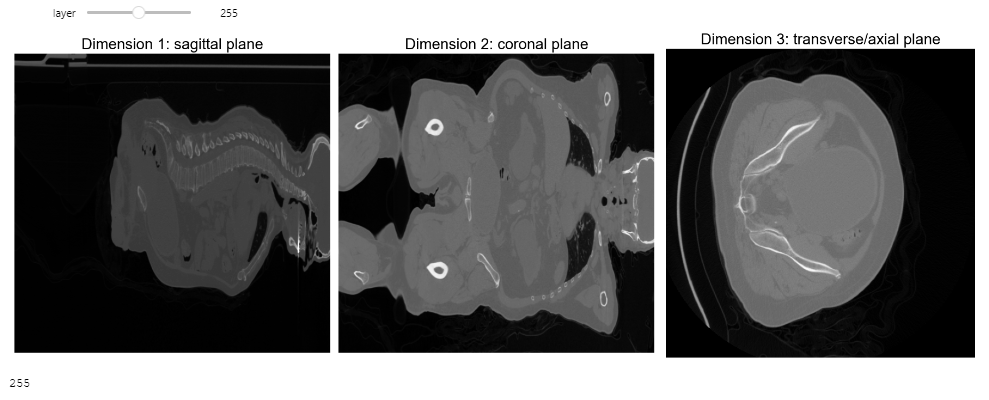
\includegraphics{images/slider1.PNG}
\caption{Slider1}
\end{figure}

    From a sagittal and coronal view, the image appears to be squished. The
voxels (Pixels in 2D \(\approx\) Voxels in 3D) must therefore be scaled.

    \begin{tcolorbox}[breakable, size=fbox, boxrule=1pt, pad at break*=1mm,colback=cellbackground, colframe=cellborder]
\prompt{In}{incolor}{4}{\boxspacing}
\begin{Verbatim}[commandchars=\\\{\}]
\PY{k}{def} \PY{n+nf}{explore\PYZus{}seg\PYZus{}image}\PY{p}{(}\PY{n}{layer}\PY{p}{)}\PY{p}{:}
    \PY{n}{fig}\PY{p}{,} \PY{n}{axs} \PY{o}{=} \PY{n}{plt}\PY{o}{.}\PY{n}{subplots}\PY{p}{(}\PY{l+m+mi}{1}\PY{p}{,} \PY{l+m+mi}{3}\PY{p}{,} \PY{n}{figsize}\PY{o}{=}\PY{p}{(}\PY{l+m+mi}{18}\PY{p}{,} \PY{l+m+mi}{6}\PY{p}{)}\PY{p}{)}  
    \PY{n}{panes} \PY{o}{=} \PY{p}{[}\PY{l+s+s1}{\PYZsq{}}\PY{l+s+s1}{sagittal}\PY{l+s+s1}{\PYZsq{}}\PY{p}{,} \PY{l+s+s1}{\PYZsq{}}\PY{l+s+s1}{coronal}\PY{l+s+s1}{\PYZsq{}}\PY{p}{,} \PY{l+s+s1}{\PYZsq{}}\PY{l+s+s1}{transverse/axial}\PY{l+s+s1}{\PYZsq{}}\PY{p}{]}
    \PY{n}{mtx} \PY{o}{=} \PY{n}{seg\PYZus{}mtx}
    \PY{k}{for} \PY{n}{dim} \PY{o+ow}{in} \PY{n+nb}{range}\PY{p}{(}\PY{n+nb}{len}\PY{p}{(}\PY{n}{mtx}\PY{o}{.}\PY{n}{shape}\PY{p}{)}\PY{p}{)}\PY{p}{:}
        \PY{k}{if} \PY{n}{dim} \PY{o}{==} \PY{l+m+mi}{0}\PY{p}{:}
            \PY{n}{axs}\PY{p}{[}\PY{n}{dim}\PY{p}{]}\PY{o}{.}\PY{n}{imshow}\PY{p}{(}\PY{n}{mtx}\PY{p}{[}\PY{n}{layer}\PY{p}{,} \PY{p}{:}\PY{p}{,} \PY{p}{:}\PY{p}{]}\PY{p}{,} \PY{n}{cmap}\PY{o}{=}\PY{l+s+s1}{\PYZsq{}}\PY{l+s+s1}{gray}\PY{l+s+s1}{\PYZsq{}}\PY{p}{)}
        \PY{k}{elif} \PY{n}{dim} \PY{o}{==} \PY{l+m+mi}{1}\PY{p}{:}
            \PY{n}{axs}\PY{p}{[}\PY{n}{dim}\PY{p}{]}\PY{o}{.}\PY{n}{imshow}\PY{p}{(}\PY{n}{mtx}\PY{p}{[}\PY{p}{:}\PY{p}{,} \PY{n}{layer}\PY{p}{,} \PY{p}{:}\PY{p}{]}\PY{p}{,} \PY{n}{cmap}\PY{o}{=}\PY{l+s+s1}{\PYZsq{}}\PY{l+s+s1}{gray}\PY{l+s+s1}{\PYZsq{}}\PY{p}{)}
        \PY{k}{else}\PY{p}{:}
            \PY{n}{axs}\PY{p}{[}\PY{n}{dim}\PY{p}{]}\PY{o}{.}\PY{n}{imshow}\PY{p}{(}\PY{n}{mtx}\PY{p}{[}\PY{p}{:}\PY{p}{,} \PY{p}{:}\PY{p}{,} \PY{n}{layer}\PY{p}{]}\PY{p}{,} \PY{n}{cmap}\PY{o}{=}\PY{l+s+s1}{\PYZsq{}}\PY{l+s+s1}{gray}\PY{l+s+s1}{\PYZsq{}}\PY{p}{)}

        \PY{n}{axs}\PY{p}{[}\PY{n}{dim}\PY{p}{]}\PY{o}{.}\PY{n}{set\PYZus{}title}\PY{p}{(}\PY{l+s+sa}{f}\PY{l+s+s2}{\PYZdq{}}\PY{l+s+s2}{Dimension }\PY{l+s+si}{\PYZob{}}\PY{n}{dim}\PY{o}{+}\PY{l+m+mi}{1}\PY{l+s+si}{\PYZcb{}}\PY{l+s+s2}{: }\PY{l+s+si}{\PYZob{}}\PY{n}{panes}\PY{p}{[}\PY{n}{dim}\PY{p}{]}\PY{l+s+si}{\PYZcb{}}\PY{l+s+s2}{ plane}\PY{l+s+s2}{\PYZdq{}}\PY{p}{,} \PY{n}{family}\PY{o}{=}\PY{l+s+s1}{\PYZsq{}}\PY{l+s+s1}{Arial}\PY{l+s+s1}{\PYZsq{}}\PY{p}{,} \PY{n}{fontsize}\PY{o}{=}\PY{l+m+mi}{20}\PY{p}{)}
        \PY{n}{axs}\PY{p}{[}\PY{n}{dim}\PY{p}{]}\PY{o}{.}\PY{n}{axis}\PY{p}{(}\PY{l+s+s1}{\PYZsq{}}\PY{l+s+s1}{off}\PY{l+s+s1}{\PYZsq{}}\PY{p}{)}
        
    \PY{n}{plt}\PY{o}{.}\PY{n}{tight\PYZus{}layout}\PY{p}{(}\PY{p}{)}

    \PY{k}{return} \PY{n}{layer}


\PY{n}{interact}\PY{p}{(}\PY{n}{explore\PYZus{}seg\PYZus{}image}\PY{p}{,} \PY{n}{layer}\PY{o}{=}\PY{p}{(}\PY{l+m+mi}{0}\PY{p}{,} \PY{n+nb}{min}\PY{p}{(}\PY{n}{seg\PYZus{}mtx}\PY{o}{.}\PY{n}{shape}\PY{p}{[}\PY{l+m+mi}{2}\PY{p}{]}\PY{o}{\PYZhy{}}\PY{l+m+mi}{1}\PY{p}{,} \PY{n}{seg\PYZus{}mtx}\PY{o}{.}\PY{n}{shape}\PY{p}{[}\PY{l+m+mi}{1}\PY{p}{]}\PY{o}{\PYZhy{}}\PY{l+m+mi}{1}\PY{p}{)}\PY{p}{)}\PY{p}{)}
\end{Verbatim}
\end{tcolorbox}

    
    \begin{Verbatim}[commandchars=\\\{\}]
interactive(children=(IntSlider(value=255, description='layer', max=511), Output()), \_dom\_classes=('widget-int…
    \end{Verbatim}

    
            \begin{tcolorbox}[breakable, size=fbox, boxrule=.5pt, pad at break*=1mm, opacityfill=0]
\prompt{Out}{outcolor}{4}{\boxspacing}
\begin{Verbatim}[commandchars=\\\{\}]
<function \_\_main\_\_.explore\_seg\_image(layer)>
\end{Verbatim}
\end{tcolorbox}
        
    \begin{figure}
\centering
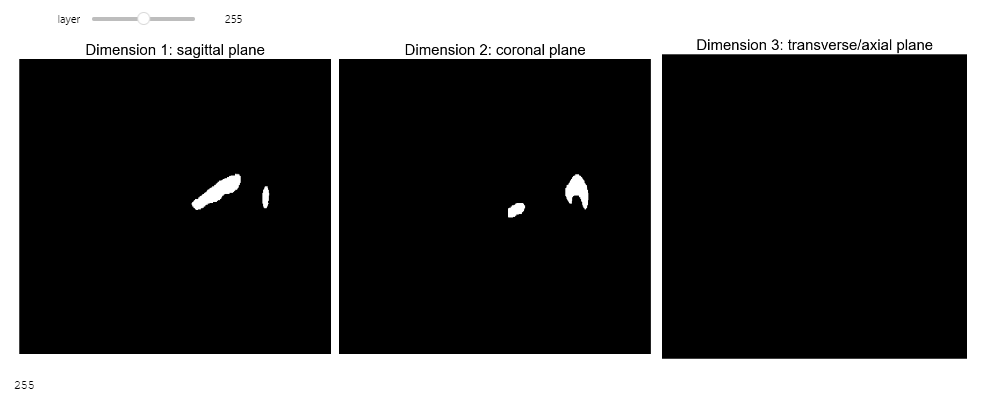
\includegraphics{images/slider2.PNG}
\caption{Slider2}
\end{figure}

    \hypertarget{task-1}{%
\section{Task 1}\label{task-1}}

    \hypertarget{a-load-the-ct-image-resample-the-image-to-an-isotropic-resolution-of-3x3x3mm}{%
\subsubsection{\texorpdfstring{a) Load the CT image, resample the image
to an isotropic \(^*\) resolution of
3x3x3mm}{a) Load the CT image, resample the image to an isotropic \^{}* resolution of 3x3x3mm}}\label{a-load-the-ct-image-resample-the-image-to-an-isotropic-resolution-of-3x3x3mm}}

\(^*\) isotropic \(=\) same in all directions \ldots{} meaning, that all
dimensions should be of the same scale

    \begin{tcolorbox}[breakable, size=fbox, boxrule=1pt, pad at break*=1mm,colback=cellbackground, colframe=cellborder]
\prompt{In}{incolor}{5}{\boxspacing}
\begin{Verbatim}[commandchars=\\\{\}]
\PY{n}{new\PYZus{}voxel\PYZus{}size} \PY{o}{=} \PY{p}{[}\PY{l+m+mi}{3}\PY{p}{,} \PY{l+m+mi}{3}\PY{p}{,} \PY{l+m+mi}{3}\PY{p}{]}

\PY{c+c1}{\PYZsh{} resample and safe image iff not done yet}
\PY{k}{try}\PY{p}{:}
    \PY{n}{resampled\PYZus{}mtx} \PY{o}{=} \PY{n}{resampled\PYZus{}img}\PY{o}{.}\PY{n}{get\PYZus{}fdata}\PY{p}{(}\PY{p}{)}
\PY{k}{except} \PY{n+ne}{NameError}\PY{p}{:}
    \PY{n+nb}{print}\PY{p}{(}\PY{l+s+s2}{\PYZdq{}}\PY{l+s+s2}{Resampling image...}\PY{l+s+s2}{\PYZdq{}}\PY{p}{)}
    \PY{n}{resampled\PYZus{}img} \PY{o}{=} \PY{n}{resample\PYZus{}img}\PY{p}{(}\PY{n}{ct\PYZus{}img}\PY{p}{,} \PY{n}{target\PYZus{}affine}\PY{o}{=}\PY{n}{np}\PY{o}{.}\PY{n}{diag}\PY{p}{(}\PY{n}{new\PYZus{}voxel\PYZus{}size}\PY{p}{)}\PY{p}{,} \PY{n}{interpolation}\PY{o}{=}\PY{l+s+s1}{\PYZsq{}}\PY{l+s+s1}{nearest}\PY{l+s+s1}{\PYZsq{}}\PY{p}{)}
    \PY{n}{nib}\PY{o}{.}\PY{n}{save}\PY{p}{(}\PY{n}{resampled\PYZus{}img}\PY{p}{,} \PY{l+s+s1}{\PYZsq{}}\PY{l+s+s1}{data/resampled\PYZus{}CT.nii.gz}\PY{l+s+s1}{\PYZsq{}}\PY{p}{)}
    \PY{n}{resampled\PYZus{}img} \PY{o}{=} \PY{n}{nib}\PY{o}{.}\PY{n}{load}\PY{p}{(}\PY{l+s+s1}{\PYZsq{}}\PY{l+s+s1}{data/resampled\PYZus{}CT.nii.gz}\PY{l+s+s1}{\PYZsq{}}\PY{p}{)}
    \PY{n}{resampled\PYZus{}mtx} \PY{o}{=} \PY{n}{resampled\PYZus{}img}\PY{o}{.}\PY{n}{get\PYZus{}fdata}\PY{p}{(}\PY{p}{)}



\PY{k}{def} \PY{n+nf}{explore\PYZus{}resampled\PYZus{}image}\PY{p}{(}\PY{n}{layer1}\PY{p}{,} \PY{n}{layer2}\PY{p}{)}\PY{p}{:}
    \PY{n}{fig}\PY{p}{,} \PY{n}{axs} \PY{o}{=} \PY{n}{plt}\PY{o}{.}\PY{n}{subplots}\PY{p}{(}\PY{l+m+mi}{1}\PY{p}{,} \PY{l+m+mi}{3}\PY{p}{,} \PY{n}{figsize}\PY{o}{=}\PY{p}{(}\PY{l+m+mi}{18}\PY{p}{,} \PY{l+m+mi}{6}\PY{p}{)}\PY{p}{)}  
    \PY{n}{panes} \PY{o}{=} \PY{p}{[}\PY{l+s+s1}{\PYZsq{}}\PY{l+s+s1}{sagittal}\PY{l+s+s1}{\PYZsq{}}\PY{p}{,} \PY{l+s+s1}{\PYZsq{}}\PY{l+s+s1}{coronal}\PY{l+s+s1}{\PYZsq{}}\PY{p}{,} \PY{l+s+s1}{\PYZsq{}}\PY{l+s+s1}{transverse/axial}\PY{l+s+s1}{\PYZsq{}}\PY{p}{]}
    \PY{n}{mtx} \PY{o}{=} \PY{n}{resampled\PYZus{}mtx}
    \PY{n}{cmap} \PY{o}{=} \PY{l+s+s1}{\PYZsq{}}\PY{l+s+s1}{gray}\PY{l+s+s1}{\PYZsq{}}
    \PY{k}{for} \PY{n}{dim} \PY{o+ow}{in} \PY{n+nb}{range}\PY{p}{(}\PY{n+nb}{len}\PY{p}{(}\PY{n}{mtx}\PY{o}{.}\PY{n}{shape}\PY{p}{)}\PY{p}{)}\PY{p}{:}
        \PY{k}{if} \PY{n}{dim} \PY{o}{==} \PY{l+m+mi}{0}\PY{p}{:}
            \PY{n}{axs}\PY{p}{[}\PY{n}{dim}\PY{p}{]}\PY{o}{.}\PY{n}{imshow}\PY{p}{(}\PY{n}{mtx}\PY{p}{[}\PY{n}{layer1}\PY{p}{,} \PY{p}{:}\PY{p}{,} \PY{p}{:}\PY{p}{]}\PY{p}{,} \PY{n}{cmap}\PY{o}{=}\PY{n}{cmap}\PY{p}{)}
        \PY{k}{elif} \PY{n}{dim} \PY{o}{==} \PY{l+m+mi}{1}\PY{p}{:}
            \PY{n}{axs}\PY{p}{[}\PY{n}{dim}\PY{p}{]}\PY{o}{.}\PY{n}{imshow}\PY{p}{(}\PY{n}{mtx}\PY{p}{[}\PY{p}{:}\PY{p}{,} \PY{n}{layer1}\PY{p}{,} \PY{p}{:}\PY{p}{]}\PY{p}{,} \PY{n}{cmap}\PY{o}{=}\PY{n}{cmap}\PY{p}{)}
        \PY{k}{else}\PY{p}{:}
            \PY{n}{axs}\PY{p}{[}\PY{n}{dim}\PY{p}{]}\PY{o}{.}\PY{n}{imshow}\PY{p}{(}\PY{n}{mtx}\PY{p}{[}\PY{p}{:}\PY{p}{,} \PY{p}{:}\PY{p}{,} \PY{n}{layer2}\PY{p}{]}\PY{p}{,} \PY{n}{cmap}\PY{o}{=}\PY{n}{cmap}\PY{p}{)}

        \PY{n}{axs}\PY{p}{[}\PY{n}{dim}\PY{p}{]}\PY{o}{.}\PY{n}{set\PYZus{}title}\PY{p}{(}\PY{l+s+sa}{f}\PY{l+s+s2}{\PYZdq{}}\PY{l+s+s2}{Dimension }\PY{l+s+si}{\PYZob{}}\PY{n}{dim}\PY{o}{+}\PY{l+m+mi}{1}\PY{l+s+si}{\PYZcb{}}\PY{l+s+s2}{: }\PY{l+s+si}{\PYZob{}}\PY{n}{panes}\PY{p}{[}\PY{n}{dim}\PY{p}{]}\PY{l+s+si}{\PYZcb{}}\PY{l+s+s2}{ plane}\PY{l+s+s2}{\PYZdq{}}\PY{p}{,} \PY{n}{family}\PY{o}{=}\PY{l+s+s1}{\PYZsq{}}\PY{l+s+s1}{Arial}\PY{l+s+s1}{\PYZsq{}}\PY{p}{,} \PY{n}{fontsize}\PY{o}{=}\PY{l+m+mi}{20}\PY{p}{)}
        \PY{n}{axs}\PY{p}{[}\PY{n}{dim}\PY{p}{]}\PY{o}{.}\PY{n}{axis}\PY{p}{(}\PY{l+s+s1}{\PYZsq{}}\PY{l+s+s1}{off}\PY{l+s+s1}{\PYZsq{}}\PY{p}{)}
        
    \PY{n}{plt}\PY{o}{.}\PY{n}{tight\PYZus{}layout}\PY{p}{(}\PY{p}{)}

    \PY{k}{return} \PY{n}{layer1}\PY{p}{,} \PY{n}{layer2}

\PY{n}{interact}\PY{p}{(}\PY{n}{explore\PYZus{}resampled\PYZus{}image}\PY{p}{,} \PY{n}{layer1}\PY{o}{=}\PY{p}{(}\PY{l+m+mi}{0}\PY{p}{,} \PY{n+nb}{min}\PY{p}{(}\PY{n}{resampled\PYZus{}mtx}\PY{o}{.}\PY{n}{shape}\PY{p}{[}\PY{l+m+mi}{0}\PY{p}{]}\PY{o}{\PYZhy{}}\PY{l+m+mi}{1}\PY{p}{,} \PY{n}{resampled\PYZus{}mtx}\PY{o}{.}\PY{n}{shape}\PY{p}{[}\PY{l+m+mi}{1}\PY{p}{]}\PY{o}{\PYZhy{}}\PY{l+m+mi}{1}\PY{p}{)}\PY{p}{)}\PY{p}{,} \PY{n}{layer2}\PY{o}{=}\PY{p}{(}\PY{l+m+mi}{0}\PY{p}{,} \PY{n}{resampled\PYZus{}mtx}\PY{o}{.}\PY{n}{shape}\PY{p}{[}\PY{l+m+mi}{2}\PY{p}{]}\PY{o}{\PYZhy{}}\PY{l+m+mi}{1}\PY{p}{)}\PY{p}{)}
\end{Verbatim}
\end{tcolorbox}

    \begin{Verbatim}[commandchars=\\\{\}]
Resampling image{\ldots}
    \end{Verbatim}

    
    \begin{Verbatim}[commandchars=\\\{\}]
interactive(children=(IntSlider(value=80, description='layer1', max=161), IntSlider(value=225, description='la…
    \end{Verbatim}

    
            \begin{tcolorbox}[breakable, size=fbox, boxrule=.5pt, pad at break*=1mm, opacityfill=0]
\prompt{Out}{outcolor}{5}{\boxspacing}
\begin{Verbatim}[commandchars=\\\{\}]
<function \_\_main\_\_.explore\_resampled\_image(layer1, layer2)>
\end{Verbatim}
\end{tcolorbox}
        
    \begin{figure}
\centering
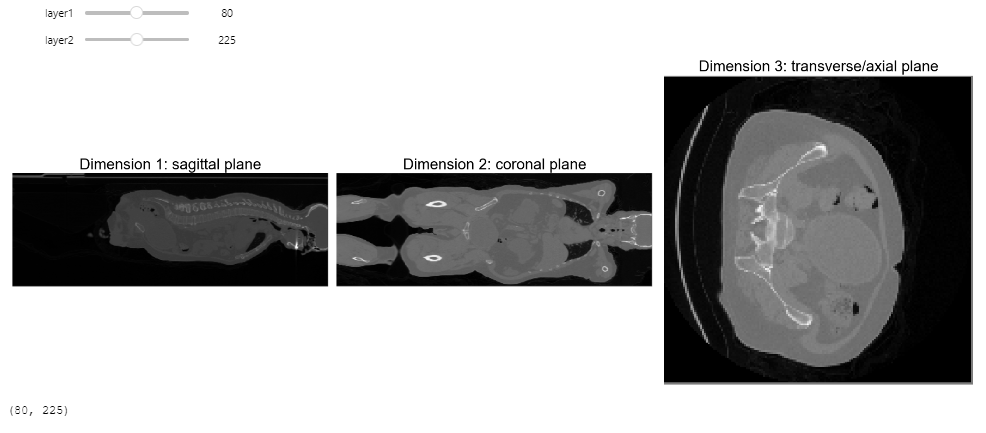
\includegraphics{images/slider3.PNG}
\caption{Slider3}
\end{figure}

    \hypertarget{b-create-one-maximum-intensity-projection-mip-along-the-coronal-axis-and-one-mip-along-the-sagittal-axis}{%
\subsubsection{b) Create one maximum intensity projection (MIP) along
the coronal axis and one MIP along the sagittal
axis}\label{b-create-one-maximum-intensity-projection-mip-along-the-coronal-axis-and-one-mip-along-the-sagittal-axis}}

    \begin{tcolorbox}[breakable, size=fbox, boxrule=1pt, pad at break*=1mm,colback=cellbackground, colframe=cellborder]
\prompt{In}{incolor}{6}{\boxspacing}
\begin{Verbatim}[commandchars=\\\{\}]
\PY{c+c1}{\PYZsh{} arbitrary 3D array for demonstrating the amax method}
\PY{n}{arr} \PY{o}{=} \PY{n}{np}\PY{o}{.}\PY{n}{array}\PY{p}{(}\PY{p}{[}\PY{p}{[}\PY{p}{[}\PY{l+m+mi}{1}\PY{p}{,} \PY{l+m+mi}{2}\PY{p}{,} \PY{l+m+mi}{3}\PY{p}{]}\PY{p}{,} \PY{p}{[}\PY{l+m+mi}{4}\PY{p}{,} \PY{l+m+mi}{5}\PY{p}{,} \PY{l+m+mi}{6}\PY{p}{]}\PY{p}{]}\PY{p}{,} \PY{p}{[}\PY{p}{[}\PY{l+m+mi}{7}\PY{p}{,} \PY{l+m+mi}{8}\PY{p}{,} \PY{l+m+mi}{9}\PY{p}{]}\PY{p}{,} \PY{p}{[}\PY{l+m+mi}{10}\PY{p}{,} \PY{l+m+mi}{11}\PY{p}{,} \PY{l+m+mi}{12}\PY{p}{]}\PY{p}{]}\PY{p}{]}\PY{p}{)}

\PY{n}{max\PYZus{}value\PYZus{}0} \PY{o}{=} \PY{n}{np}\PY{o}{.}\PY{n}{amax}\PY{p}{(}\PY{n}{arr}\PY{p}{,} \PY{n}{axis}\PY{o}{=}\PY{l+m+mi}{0}\PY{p}{)}
\PY{n}{max\PYZus{}value\PYZus{}1} \PY{o}{=} \PY{n}{np}\PY{o}{.}\PY{n}{amax}\PY{p}{(}\PY{n}{arr}\PY{p}{,} \PY{n}{axis}\PY{o}{=}\PY{l+m+mi}{1}\PY{p}{)}
\PY{n}{max\PYZus{}value\PYZus{}2} \PY{o}{=} \PY{n}{np}\PY{o}{.}\PY{n}{amax}\PY{p}{(}\PY{n}{arr}\PY{p}{,} \PY{n}{axis}\PY{o}{=}\PY{l+m+mi}{2}\PY{p}{)}
\PY{n}{max\PYZus{}value\PYZus{}all} \PY{o}{=} \PY{n}{np}\PY{o}{.}\PY{n}{amax}\PY{p}{(}\PY{n}{arr}\PY{p}{)}

\PY{n+nb}{print}\PY{p}{(}\PY{l+s+s2}{\PYZdq{}}\PY{l+s+s2}{Max along axis 0:}\PY{l+s+s2}{\PYZdq{}}\PY{p}{,} \PY{n}{max\PYZus{}value\PYZus{}0}\PY{p}{)}
\PY{n+nb}{print}\PY{p}{(}\PY{l+s+s2}{\PYZdq{}}\PY{l+s+s2}{Max along axis 1:}\PY{l+s+s2}{\PYZdq{}}\PY{p}{,} \PY{n}{max\PYZus{}value\PYZus{}1}\PY{p}{)}
\PY{n+nb}{print}\PY{p}{(}\PY{l+s+s2}{\PYZdq{}}\PY{l+s+s2}{Max along axis 2:}\PY{l+s+s2}{\PYZdq{}}\PY{p}{,} \PY{n}{max\PYZus{}value\PYZus{}2}\PY{p}{)}
\PY{n+nb}{print}\PY{p}{(}\PY{l+s+s2}{\PYZdq{}}\PY{l+s+s2}{Max of all elements:}\PY{l+s+s2}{\PYZdq{}}\PY{p}{,} \PY{n}{max\PYZus{}value\PYZus{}all}\PY{p}{)}
\end{Verbatim}
\end{tcolorbox}

    \begin{Verbatim}[commandchars=\\\{\}]
Max along axis 0: [[ 7  8  9]
 [10 11 12]]
Max along axis 1: [[ 4  5  6]
 [10 11 12]]
Max along axis 2: [[ 3  6]
 [ 9 12]]
Max of all elements: 12
    \end{Verbatim}

    \begin{tcolorbox}[breakable, size=fbox, boxrule=1pt, pad at break*=1mm,colback=cellbackground, colframe=cellborder]
\prompt{In}{incolor}{7}{\boxspacing}
\begin{Verbatim}[commandchars=\\\{\}]
\PY{c+c1}{\PYZsh{} header contains image metadata}
\PY{n}{ct\PYZus{}zoom} \PY{o}{=} \PY{n}{ct\PYZus{}img}\PY{o}{.}\PY{n}{header}\PY{o}{.}\PY{n}{get\PYZus{}zooms}\PY{p}{(}\PY{p}{)}
\PY{n}{resampled\PYZus{}zoom} \PY{o}{=} \PY{n}{resampled\PYZus{}img}\PY{o}{.}\PY{n}{header}\PY{o}{.}\PY{n}{get\PYZus{}zooms}\PY{p}{(}\PY{p}{)}
\PY{n+nb}{print}\PY{p}{(}\PY{l+s+sa}{f}\PY{l+s+s2}{\PYZdq{}}\PY{l+s+s2}{Original voxel sizes in mm: }\PY{l+s+si}{\PYZob{}}\PY{n}{ct\PYZus{}zoom}\PY{l+s+si}{\PYZcb{}}\PY{l+s+se}{\PYZbs{}n}\PY{l+s+s2}{Resampled voxel sizes in mm: }\PY{l+s+si}{\PYZob{}}\PY{n}{resampled\PYZus{}zoom}\PY{l+s+si}{\PYZcb{}}\PY{l+s+s2}{\PYZdq{}}\PY{p}{)}


\PY{n}{mip\PYZus{}sagittal} \PY{o}{=} \PY{n}{np}\PY{o}{.}\PY{n}{amax}\PY{p}{(}\PY{n}{resampled\PYZus{}mtx}\PY{p}{,} \PY{n}{axis}\PY{o}{=}\PY{l+m+mi}{0}\PY{p}{)}
\PY{n}{mip\PYZus{}coronal} \PY{o}{=} \PY{n}{np}\PY{o}{.}\PY{n}{amax}\PY{p}{(}\PY{n}{resampled\PYZus{}mtx}\PY{p}{,} \PY{n}{axis}\PY{o}{=}\PY{l+m+mi}{1}\PY{p}{)}

\PY{n}{fig}\PY{p}{,} \PY{n}{axs} \PY{o}{=} \PY{n}{plt}\PY{o}{.}\PY{n}{subplots}\PY{p}{(}\PY{l+m+mi}{2}\PY{p}{,} \PY{l+m+mi}{1}\PY{p}{,} \PY{n}{figsize}\PY{o}{=}\PY{p}{(}\PY{l+m+mi}{12}\PY{p}{,} \PY{l+m+mi}{6}\PY{p}{)}\PY{p}{)}


\PY{n}{axs}\PY{p}{[}\PY{l+m+mi}{0}\PY{p}{]}\PY{o}{.}\PY{n}{imshow}\PY{p}{(}\PY{n}{mip\PYZus{}coronal}\PY{p}{,} \PY{n}{cmap}\PY{o}{=}\PY{l+s+s1}{\PYZsq{}}\PY{l+s+s1}{gray}\PY{l+s+s1}{\PYZsq{}}\PY{p}{)}
\PY{n}{axs}\PY{p}{[}\PY{l+m+mi}{0}\PY{p}{]}\PY{o}{.}\PY{n}{set\PYZus{}title}\PY{p}{(}\PY{l+s+s2}{\PYZdq{}}\PY{l+s+s2}{MIP \PYZhy{} Coronal}\PY{l+s+s2}{\PYZdq{}}\PY{p}{)}
\PY{n}{axs}\PY{p}{[}\PY{l+m+mi}{0}\PY{p}{]}\PY{o}{.}\PY{n}{axis}\PY{p}{(}\PY{l+s+s1}{\PYZsq{}}\PY{l+s+s1}{off}\PY{l+s+s1}{\PYZsq{}}\PY{p}{)}

\PY{n}{axs}\PY{p}{[}\PY{l+m+mi}{1}\PY{p}{]}\PY{o}{.}\PY{n}{imshow}\PY{p}{(}\PY{n}{mip\PYZus{}sagittal}\PY{p}{,} \PY{n}{cmap}\PY{o}{=}\PY{l+s+s1}{\PYZsq{}}\PY{l+s+s1}{gray}\PY{l+s+s1}{\PYZsq{}}\PY{p}{)}
\PY{n}{axs}\PY{p}{[}\PY{l+m+mi}{1}\PY{p}{]}\PY{o}{.}\PY{n}{set\PYZus{}title}\PY{p}{(}\PY{l+s+s2}{\PYZdq{}}\PY{l+s+s2}{MIP \PYZhy{} Sagittal}\PY{l+s+s2}{\PYZdq{}}\PY{p}{)}
\PY{n}{axs}\PY{p}{[}\PY{l+m+mi}{1}\PY{p}{]}\PY{o}{.}\PY{n}{axis}\PY{p}{(}\PY{l+s+s1}{\PYZsq{}}\PY{l+s+s1}{off}\PY{l+s+s1}{\PYZsq{}}\PY{p}{)}

\PY{n}{plt}\PY{o}{.}\PY{n}{show}\PY{p}{(}\PY{p}{)}
\end{Verbatim}
\end{tcolorbox}

    \begin{Verbatim}[commandchars=\\\{\}]
Original voxel sizes in mm: (0.9433594, 0.9433594, 2.5)
Resampled voxel sizes in mm: (3.0, 3.0, 3.0)
    \end{Verbatim}

    \begin{center}
    \adjustimage{max size={0.9\linewidth}{0.9\paperheight}}{development_files/development_18_1.png}
    \end{center}
    { \hspace*{\fill} \\}
    
    \hypertarget{c-save-the-resulting-images-as-png-file-with-at-least-400-dp}{%
\subsubsection{c) Save the resulting images as PNG file with at least
400
dp}\label{c-save-the-resulting-images-as-png-file-with-at-least-400-dp}}

    \begin{tcolorbox}[breakable, size=fbox, boxrule=1pt, pad at break*=1mm,colback=cellbackground, colframe=cellborder]
\prompt{In}{incolor}{8}{\boxspacing}
\begin{Verbatim}[commandchars=\\\{\}]
\PY{n}{DPI} \PY{o}{=} \PY{l+m+mi}{600} 
\PY{k}{assert} \PY{n}{DPI} \PY{o}{\PYZgt{}}\PY{o}{=} \PY{l+m+mi}{400}\PY{p}{,} \PY{l+s+s2}{\PYZdq{}}\PY{l+s+s2}{DPI should be at least 400 for high quality images}\PY{l+s+s2}{\PYZdq{}}

\PY{n}{fig}\PY{p}{,} \PY{n}{ax} \PY{o}{=} \PY{n}{plt}\PY{o}{.}\PY{n}{subplots}\PY{p}{(}\PY{n}{figsize}\PY{o}{=}\PY{p}{(}\PY{l+m+mi}{5}\PY{p}{,} \PY{l+m+mi}{5}\PY{p}{)}\PY{p}{)}
\PY{n}{ax}\PY{o}{.}\PY{n}{imshow}\PY{p}{(}\PY{n}{mip\PYZus{}coronal}\PY{p}{,} \PY{n}{cmap}\PY{o}{=}\PY{l+s+s1}{\PYZsq{}}\PY{l+s+s1}{gray}\PY{l+s+s1}{\PYZsq{}}\PY{p}{)}
\PY{n}{ax}\PY{o}{.}\PY{n}{set\PYZus{}title}\PY{p}{(}\PY{l+s+s2}{\PYZdq{}}\PY{l+s+s2}{MIP \PYZhy{} Coronal}\PY{l+s+s2}{\PYZdq{}}\PY{p}{)}
\PY{n}{ax}\PY{o}{.}\PY{n}{axis}\PY{p}{(}\PY{l+s+s1}{\PYZsq{}}\PY{l+s+s1}{off}\PY{l+s+s1}{\PYZsq{}}\PY{p}{)}
\PY{n}{fig}\PY{o}{.}\PY{n}{savefig}\PY{p}{(}\PY{l+s+s2}{\PYZdq{}}\PY{l+s+s2}{images/mip\PYZus{}coronal.png}\PY{l+s+s2}{\PYZdq{}}\PY{p}{,} \PY{n}{dpi}\PY{o}{=}\PY{l+m+mi}{600}\PY{p}{)}


\PY{n}{fig}\PY{p}{,} \PY{n}{ax} \PY{o}{=} \PY{n}{plt}\PY{o}{.}\PY{n}{subplots}\PY{p}{(}\PY{n}{figsize}\PY{o}{=}\PY{p}{(}\PY{l+m+mi}{5}\PY{p}{,} \PY{l+m+mi}{5}\PY{p}{)}\PY{p}{)}
\PY{n}{ax}\PY{o}{.}\PY{n}{imshow}\PY{p}{(}\PY{n}{mip\PYZus{}sagittal}\PY{p}{,} \PY{n}{cmap}\PY{o}{=}\PY{l+s+s1}{\PYZsq{}}\PY{l+s+s1}{gray}\PY{l+s+s1}{\PYZsq{}}\PY{p}{)}
\PY{n}{ax}\PY{o}{.}\PY{n}{set\PYZus{}title}\PY{p}{(}\PY{l+s+s2}{\PYZdq{}}\PY{l+s+s2}{MIP \PYZhy{} Sagittal}\PY{l+s+s2}{\PYZdq{}}\PY{p}{)}
\PY{n}{ax}\PY{o}{.}\PY{n}{axis}\PY{p}{(}\PY{l+s+s1}{\PYZsq{}}\PY{l+s+s1}{off}\PY{l+s+s1}{\PYZsq{}}\PY{p}{)}
\PY{n}{fig}\PY{o}{.}\PY{n}{savefig}\PY{p}{(}\PY{l+s+s2}{\PYZdq{}}\PY{l+s+s2}{images/mip\PYZus{}sagittal.png}\PY{l+s+s2}{\PYZdq{}}\PY{p}{,} \PY{n}{dpi}\PY{o}{=}\PY{l+m+mi}{600}\PY{p}{)}
\end{Verbatim}
\end{tcolorbox}

    \begin{center}
    \adjustimage{max size={0.9\linewidth}{0.9\paperheight}}{development_files/development_20_0.png}
    \end{center}
    { \hspace*{\fill} \\}
    
    \begin{center}
    \adjustimage{max size={0.9\linewidth}{0.9\paperheight}}{development_files/development_20_1.png}
    \end{center}
    { \hspace*{\fill} \\}
    
    np.amax: np.amax is a function from the NumPy library that computes the
maximum value along a specified axis of an array.

In the code, np.amax is used to compute the maximum intensity projection
(MIP) along the coronal and sagittal axes of the resampled CT image. By
specifying axis=0 and axis=1, respectively, we calculate the maximum
intensity projection along the coronal and sagittal axes. This operation
effectively collapses the 3D image along the specified axes, resulting
in 2D images representing the maximum intensity projection.

    \hypertarget{little-bonus-visualizing-the-aorta-in-the-ct-scan}{%
\subsubsection{Little Bonus: Visualizing the aorta in the
CT-scan}\label{little-bonus-visualizing-the-aorta-in-the-ct-scan}}

    \begin{tcolorbox}[breakable, size=fbox, boxrule=1pt, pad at break*=1mm,colback=cellbackground, colframe=cellborder]
\prompt{In}{incolor}{9}{\boxspacing}
\begin{Verbatim}[commandchars=\\\{\}]
\PY{c+c1}{\PYZsh{} first, we need to resample the segmentation image to the same voxel size as the CT image}
\PY{n}{new\PYZus{}voxel\PYZus{}size} \PY{o}{=} \PY{p}{[}\PY{l+m+mi}{3}\PY{p}{,} \PY{l+m+mi}{3}\PY{p}{,} \PY{l+m+mi}{3}\PY{p}{]}

\PY{c+c1}{\PYZsh{} resample and safe image iff not done yet}
\PY{k}{try}\PY{p}{:}
    \PY{n}{resampled\PYZus{}seg\PYZus{}mtx} \PY{o}{=} \PY{n}{resampled\PYZus{}seg\PYZus{}img}\PY{o}{.}\PY{n}{get\PYZus{}fdata}\PY{p}{(}\PY{p}{)}
\PY{k}{except} \PY{n+ne}{NameError}\PY{p}{:}
    \PY{n+nb}{print}\PY{p}{(}\PY{l+s+s2}{\PYZdq{}}\PY{l+s+s2}{Resampling image...}\PY{l+s+s2}{\PYZdq{}}\PY{p}{)}
    \PY{n}{resampled\PYZus{}seg\PYZus{}img} \PY{o}{=} \PY{n}{resample\PYZus{}img}\PY{p}{(}\PY{n}{seg\PYZus{}img}\PY{p}{,} \PY{n}{target\PYZus{}affine}\PY{o}{=}\PY{n}{np}\PY{o}{.}\PY{n}{diag}\PY{p}{(}\PY{n}{new\PYZus{}voxel\PYZus{}size}\PY{p}{)}\PY{p}{,} \PY{n}{interpolation}\PY{o}{=}\PY{l+s+s1}{\PYZsq{}}\PY{l+s+s1}{nearest}\PY{l+s+s1}{\PYZsq{}}\PY{p}{)}
    \PY{n}{nib}\PY{o}{.}\PY{n}{save}\PY{p}{(}\PY{n}{resampled\PYZus{}seg\PYZus{}img}\PY{p}{,} \PY{l+s+s1}{\PYZsq{}}\PY{l+s+s1}{data/resampled\PYZus{}segmentation.nii.gz}\PY{l+s+s1}{\PYZsq{}}\PY{p}{)}
    \PY{n}{resampled\PYZus{}seg\PYZus{}img} \PY{o}{=} \PY{n}{nib}\PY{o}{.}\PY{n}{load}\PY{p}{(}\PY{l+s+s1}{\PYZsq{}}\PY{l+s+s1}{data/resampled\PYZus{}segmentation.nii.gz}\PY{l+s+s1}{\PYZsq{}}\PY{p}{)}
    \PY{n}{resampled\PYZus{}seg\PYZus{}mtx} \PY{o}{=} \PY{n}{resampled\PYZus{}seg\PYZus{}img}\PY{o}{.}\PY{n}{get\PYZus{}fdata}\PY{p}{(}\PY{p}{)}



\PY{k}{def} \PY{n+nf}{explore\PYZus{}resampled\PYZus{}image}\PY{p}{(}\PY{n}{layer1}\PY{p}{,} \PY{n}{layer2}\PY{p}{)}\PY{p}{:}
    \PY{n}{fig}\PY{p}{,} \PY{n}{axs} \PY{o}{=} \PY{n}{plt}\PY{o}{.}\PY{n}{subplots}\PY{p}{(}\PY{l+m+mi}{1}\PY{p}{,} \PY{l+m+mi}{3}\PY{p}{,} \PY{n}{figsize}\PY{o}{=}\PY{p}{(}\PY{l+m+mi}{18}\PY{p}{,} \PY{l+m+mi}{6}\PY{p}{)}\PY{p}{)}  
    \PY{n}{panes} \PY{o}{=} \PY{p}{[}\PY{l+s+s1}{\PYZsq{}}\PY{l+s+s1}{sagittal}\PY{l+s+s1}{\PYZsq{}}\PY{p}{,} \PY{l+s+s1}{\PYZsq{}}\PY{l+s+s1}{coronal}\PY{l+s+s1}{\PYZsq{}}\PY{p}{,} \PY{l+s+s1}{\PYZsq{}}\PY{l+s+s1}{transverse/axial}\PY{l+s+s1}{\PYZsq{}}\PY{p}{]}
    \PY{n}{mtx} \PY{o}{=} \PY{n}{resampled\PYZus{}seg\PYZus{}mtx}
    \PY{n}{cmap} \PY{o}{=} \PY{l+s+s1}{\PYZsq{}}\PY{l+s+s1}{gray}\PY{l+s+s1}{\PYZsq{}}
    \PY{k}{for} \PY{n}{dim} \PY{o+ow}{in} \PY{n+nb}{range}\PY{p}{(}\PY{n+nb}{len}\PY{p}{(}\PY{n}{mtx}\PY{o}{.}\PY{n}{shape}\PY{p}{)}\PY{p}{)}\PY{p}{:}
        \PY{k}{if} \PY{n}{dim} \PY{o}{==} \PY{l+m+mi}{0}\PY{p}{:}
            \PY{n}{axs}\PY{p}{[}\PY{n}{dim}\PY{p}{]}\PY{o}{.}\PY{n}{imshow}\PY{p}{(}\PY{n}{mtx}\PY{p}{[}\PY{n}{layer1}\PY{p}{,} \PY{p}{:}\PY{p}{,} \PY{p}{:}\PY{p}{]}\PY{p}{,} \PY{n}{cmap}\PY{o}{=}\PY{n}{cmap}\PY{p}{)}
        \PY{k}{elif} \PY{n}{dim} \PY{o}{==} \PY{l+m+mi}{1}\PY{p}{:}
            \PY{n}{axs}\PY{p}{[}\PY{n}{dim}\PY{p}{]}\PY{o}{.}\PY{n}{imshow}\PY{p}{(}\PY{n}{mtx}\PY{p}{[}\PY{p}{:}\PY{p}{,} \PY{n}{layer1}\PY{p}{,} \PY{p}{:}\PY{p}{]}\PY{p}{,} \PY{n}{cmap}\PY{o}{=}\PY{n}{cmap}\PY{p}{)}
        \PY{k}{else}\PY{p}{:}
            \PY{n}{axs}\PY{p}{[}\PY{n}{dim}\PY{p}{]}\PY{o}{.}\PY{n}{imshow}\PY{p}{(}\PY{n}{mtx}\PY{p}{[}\PY{p}{:}\PY{p}{,} \PY{p}{:}\PY{p}{,} \PY{n}{layer2}\PY{p}{]}\PY{p}{,} \PY{n}{cmap}\PY{o}{=}\PY{n}{cmap}\PY{p}{)}

        \PY{n}{axs}\PY{p}{[}\PY{n}{dim}\PY{p}{]}\PY{o}{.}\PY{n}{set\PYZus{}title}\PY{p}{(}\PY{l+s+sa}{f}\PY{l+s+s2}{\PYZdq{}}\PY{l+s+s2}{Dimension }\PY{l+s+si}{\PYZob{}}\PY{n}{dim}\PY{o}{+}\PY{l+m+mi}{1}\PY{l+s+si}{\PYZcb{}}\PY{l+s+s2}{: }\PY{l+s+si}{\PYZob{}}\PY{n}{panes}\PY{p}{[}\PY{n}{dim}\PY{p}{]}\PY{l+s+si}{\PYZcb{}}\PY{l+s+s2}{ plane}\PY{l+s+s2}{\PYZdq{}}\PY{p}{,} \PY{n}{family}\PY{o}{=}\PY{l+s+s1}{\PYZsq{}}\PY{l+s+s1}{Arial}\PY{l+s+s1}{\PYZsq{}}\PY{p}{,} \PY{n}{fontsize}\PY{o}{=}\PY{l+m+mi}{20}\PY{p}{)}
        \PY{n}{axs}\PY{p}{[}\PY{n}{dim}\PY{p}{]}\PY{o}{.}\PY{n}{axis}\PY{p}{(}\PY{l+s+s1}{\PYZsq{}}\PY{l+s+s1}{off}\PY{l+s+s1}{\PYZsq{}}\PY{p}{)}
        
    \PY{n}{plt}\PY{o}{.}\PY{n}{tight\PYZus{}layout}\PY{p}{(}\PY{p}{)}

    \PY{k}{return} \PY{n}{layer1}\PY{p}{,} \PY{n}{layer2}

\PY{n}{interact}\PY{p}{(}\PY{n}{explore\PYZus{}resampled\PYZus{}image}\PY{p}{,} \PY{n}{layer1}\PY{o}{=}\PY{p}{(}\PY{l+m+mi}{0}\PY{p}{,} \PY{n+nb}{min}\PY{p}{(}\PY{n}{resampled\PYZus{}seg\PYZus{}mtx}\PY{o}{.}\PY{n}{shape}\PY{p}{[}\PY{l+m+mi}{0}\PY{p}{]}\PY{o}{\PYZhy{}}\PY{l+m+mi}{1}\PY{p}{,} \PY{n}{resampled\PYZus{}seg\PYZus{}mtx}\PY{o}{.}\PY{n}{shape}\PY{p}{[}\PY{l+m+mi}{1}\PY{p}{]}\PY{o}{\PYZhy{}}\PY{l+m+mi}{1}\PY{p}{)}\PY{p}{)}\PY{p}{,} \PY{n}{layer2}\PY{o}{=}\PY{p}{(}\PY{l+m+mi}{0}\PY{p}{,} \PY{n}{resampled\PYZus{}seg\PYZus{}mtx}\PY{o}{.}\PY{n}{shape}\PY{p}{[}\PY{l+m+mi}{2}\PY{p}{]}\PY{o}{\PYZhy{}}\PY{l+m+mi}{1}\PY{p}{)}\PY{p}{)}
\end{Verbatim}
\end{tcolorbox}

    \begin{Verbatim}[commandchars=\\\{\}]
Resampling image{\ldots}
    \end{Verbatim}

    
    \begin{Verbatim}[commandchars=\\\{\}]
interactive(children=(IntSlider(value=80, description='layer1', max=161), IntSlider(value=225, description='la…
    \end{Verbatim}

    
            \begin{tcolorbox}[breakable, size=fbox, boxrule=.5pt, pad at break*=1mm, opacityfill=0]
\prompt{Out}{outcolor}{9}{\boxspacing}
\begin{Verbatim}[commandchars=\\\{\}]
<function \_\_main\_\_.explore\_resampled\_image(layer1, layer2)>
\end{Verbatim}
\end{tcolorbox}
        
    \begin{figure}
\centering
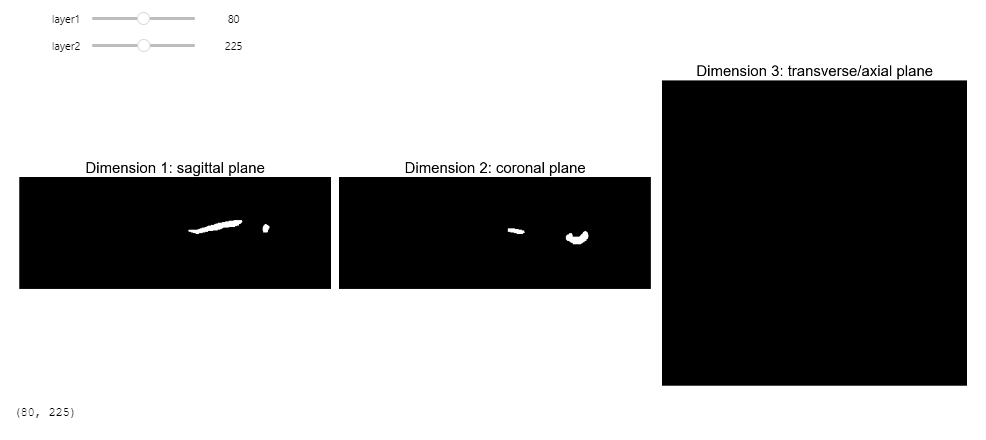
\includegraphics{images/slider4.PNG}
\caption{Slider4}
\end{figure}

    \begin{tcolorbox}[breakable, size=fbox, boxrule=1pt, pad at break*=1mm,colback=cellbackground, colframe=cellborder]
\prompt{In}{incolor}{10}{\boxspacing}
\begin{Verbatim}[commandchars=\\\{\}]
\PY{n}{img} \PY{o}{=} \PY{n}{mpimg}\PY{o}{.}\PY{n}{imread}\PY{p}{(}\PY{l+s+s1}{\PYZsq{}}\PY{l+s+s1}{images/aorta.png}\PY{l+s+s1}{\PYZsq{}}\PY{p}{)}
\PY{n}{plt}\PY{o}{.}\PY{n}{figure}\PY{p}{(}\PY{n}{figsize}\PY{o}{=}\PY{p}{(}\PY{l+m+mi}{8}\PY{p}{,}\PY{l+m+mi}{8}\PY{p}{)}\PY{p}{)}
\PY{n}{plt}\PY{o}{.}\PY{n}{imshow}\PY{p}{(}\PY{n}{img}\PY{p}{)}
\PY{n}{plt}\PY{o}{.}\PY{n}{text}\PY{p}{(}\PY{n}{x}\PY{o}{=}\PY{n}{img}\PY{o}{.}\PY{n}{shape}\PY{p}{[}\PY{l+m+mi}{1}\PY{p}{]}\PY{o}{/}\PY{o}{/}\PY{l+m+mf}{1.6}\PY{p}{,} \PY{n}{y}\PY{o}{=}\PY{n}{img}\PY{o}{.}\PY{n}{shape}\PY{p}{[}\PY{l+m+mi}{0}\PY{p}{]}\PY{p}{,} \PY{n}{s}\PY{o}{=}\PY{l+s+s1}{\PYZsq{}}\PY{l+s+s1}{Source: https://www.mcgill.ca/aorticclinic/files/aorticclinic/aortic\PYZus{}disease\PYZus{}tab.png}\PY{l+s+s1}{\PYZsq{}}\PY{p}{,} 
         \PY{n}{fontsize}\PY{o}{=}\PY{l+m+mi}{6}\PY{p}{,} \PY{n}{color}\PY{o}{=}\PY{l+s+s1}{\PYZsq{}}\PY{l+s+s1}{grey}\PY{l+s+s1}{\PYZsq{}}\PY{p}{,} \PY{n}{ha}\PY{o}{=}\PY{l+s+s1}{\PYZsq{}}\PY{l+s+s1}{center}\PY{l+s+s1}{\PYZsq{}}\PY{p}{,} \PY{n}{style}\PY{o}{=}\PY{l+s+s1}{\PYZsq{}}\PY{l+s+s1}{italic}\PY{l+s+s1}{\PYZsq{}}\PY{p}{)}
\PY{n}{plt}\PY{o}{.}\PY{n}{axis}\PY{p}{(}\PY{l+s+s1}{\PYZsq{}}\PY{l+s+s1}{off}\PY{l+s+s1}{\PYZsq{}}\PY{p}{)}
\PY{n}{plt}\PY{o}{.}\PY{n}{show}\PY{p}{(}\PY{p}{)}
\end{Verbatim}
\end{tcolorbox}

    \begin{center}
    \adjustimage{max size={0.9\linewidth}{0.9\paperheight}}{development_files/development_25_0.png}
    \end{center}
    { \hspace*{\fill} \\}
    
    \begin{tcolorbox}[breakable, size=fbox, boxrule=1pt, pad at break*=1mm,colback=cellbackground, colframe=cellborder]
\prompt{In}{incolor}{11}{\boxspacing}
\begin{Verbatim}[commandchars=\\\{\}]
\PY{c+c1}{\PYZsh{} resampled\PYZus{}img = nib.load(\PYZsq{}data/resampled\PYZus{}CT.nii.gz\PYZsq{})}
\PY{c+c1}{\PYZsh{} resampled\PYZus{}seg\PYZus{}img = nib.load(\PYZsq{}data/resampled\PYZus{}segmentation.nii.gz\PYZsq{})}
\PY{c+c1}{\PYZsh{} resampled\PYZus{}mtx = resampled\PYZus{}img.get\PYZus{}fdata()}
\PY{c+c1}{\PYZsh{} resampled\PYZus{}seg\PYZus{}mtx = resampled\PYZus{}seg\PYZus{}img.get\PYZus{}fdata()}

\PY{c+c1}{\PYZsh{} ensure the images have the same dimensions}
\PY{k}{assert} \PY{n}{resampled\PYZus{}mtx}\PY{o}{.}\PY{n}{shape} \PY{o}{==} \PY{n}{resampled\PYZus{}seg\PYZus{}mtx}\PY{o}{.}\PY{n}{shape}\PY{p}{,} \PY{l+s+s2}{\PYZdq{}}\PY{l+s+s2}{Images don}\PY{l+s+s2}{\PYZsq{}}\PY{l+s+s2}{t posess the same dimensions}\PY{l+s+s2}{\PYZdq{}}

\PY{n}{highlighted\PYZus{}mtx} \PY{o}{=} \PY{n}{np}\PY{o}{.}\PY{n}{copy}\PY{p}{(}\PY{n}{resampled\PYZus{}mtx}\PY{p}{)}

\PY{c+c1}{\PYZsh{} set intensity of the highlighted (segmented) region}
\PY{n}{highlight\PYZus{}intensity} \PY{o}{=} \PY{n}{np}\PY{o}{.}\PY{n}{max}\PY{p}{(}\PY{n}{resampled\PYZus{}mtx}\PY{p}{)}

\PY{c+c1}{\PYZsh{} iterating over the voxels }
\PY{k}{for} \PY{n}{i} \PY{o+ow}{in} \PY{n+nb}{range}\PY{p}{(}\PY{n}{resampled\PYZus{}seg\PYZus{}mtx}\PY{o}{.}\PY{n}{shape}\PY{p}{[}\PY{l+m+mi}{0}\PY{p}{]}\PY{p}{)}\PY{p}{:}
    \PY{k}{for} \PY{n}{j} \PY{o+ow}{in} \PY{n+nb}{range}\PY{p}{(}\PY{n}{resampled\PYZus{}seg\PYZus{}mtx}\PY{o}{.}\PY{n}{shape}\PY{p}{[}\PY{l+m+mi}{1}\PY{p}{]}\PY{p}{)}\PY{p}{:}
        \PY{k}{for} \PY{n}{k} \PY{o+ow}{in} \PY{n+nb}{range}\PY{p}{(}\PY{n}{resampled\PYZus{}seg\PYZus{}mtx}\PY{o}{.}\PY{n}{shape}\PY{p}{[}\PY{l+m+mi}{2}\PY{p}{]}\PY{p}{)}\PY{p}{:}
            \PY{c+c1}{\PYZsh{} if the voxel value is 1 (=white), change the corresponding voxel in the medical image to the highlight intensity}
            \PY{k}{if} \PY{n}{resampled\PYZus{}seg\PYZus{}mtx}\PY{p}{[}\PY{n}{i}\PY{p}{,} \PY{n}{j}\PY{p}{,} \PY{n}{k}\PY{p}{]} \PY{o}{==} \PY{l+m+mi}{1}\PY{p}{:}
                \PY{n}{highlighted\PYZus{}mtx}\PY{p}{[}\PY{n}{i}\PY{p}{,} \PY{n}{j}\PY{p}{,} \PY{n}{k}\PY{p}{]} \PY{o}{=} \PY{n}{highlight\PYZus{}intensity}

\PY{c+c1}{\PYZsh{} convert np array to nibabel image}
\PY{n}{highlighted\PYZus{}img} \PY{o}{=} \PY{n}{nib}\PY{o}{.}\PY{n}{Nifti1Image}\PY{p}{(}\PY{n}{highlighted\PYZus{}mtx}\PY{p}{,} \PY{n}{resampled\PYZus{}img}\PY{o}{.}\PY{n}{affine}\PY{p}{)}
\PY{n}{nib}\PY{o}{.}\PY{n}{save}\PY{p}{(}\PY{n}{highlighted\PYZus{}img}\PY{p}{,} \PY{l+s+s1}{\PYZsq{}}\PY{l+s+s1}{data/highlighted\PYZus{}resampled\PYZus{}CT.nii.gz}\PY{l+s+s1}{\PYZsq{}}\PY{p}{)}


\PY{k}{def} \PY{n+nf}{explore\PYZus{}highlighted\PYZus{}image}\PY{p}{(}\PY{n}{layer1}\PY{p}{,} \PY{n}{layer2}\PY{p}{)}\PY{p}{:}
    \PY{n}{fig}\PY{p}{,} \PY{n}{axs} \PY{o}{=} \PY{n}{plt}\PY{o}{.}\PY{n}{subplots}\PY{p}{(}\PY{l+m+mi}{1}\PY{p}{,} \PY{l+m+mi}{3}\PY{p}{,} \PY{n}{figsize}\PY{o}{=}\PY{p}{(}\PY{l+m+mi}{18}\PY{p}{,} \PY{l+m+mi}{6}\PY{p}{)}\PY{p}{)}  
    \PY{n}{panes} \PY{o}{=} \PY{p}{[}\PY{l+s+s1}{\PYZsq{}}\PY{l+s+s1}{sagittal}\PY{l+s+s1}{\PYZsq{}}\PY{p}{,} \PY{l+s+s1}{\PYZsq{}}\PY{l+s+s1}{coronal}\PY{l+s+s1}{\PYZsq{}}\PY{p}{,} \PY{l+s+s1}{\PYZsq{}}\PY{l+s+s1}{transverse/axial}\PY{l+s+s1}{\PYZsq{}}\PY{p}{]}
    \PY{n}{mtx} \PY{o}{=} \PY{n}{highlighted\PYZus{}mtx}
    \PY{n}{cmap} \PY{o}{=} \PY{l+s+s1}{\PYZsq{}}\PY{l+s+s1}{gray}\PY{l+s+s1}{\PYZsq{}}
    \PY{k}{for} \PY{n}{dim} \PY{o+ow}{in} \PY{n+nb}{range}\PY{p}{(}\PY{n+nb}{len}\PY{p}{(}\PY{n}{mtx}\PY{o}{.}\PY{n}{shape}\PY{p}{)}\PY{p}{)}\PY{p}{:}
        \PY{k}{if} \PY{n}{dim} \PY{o}{==} \PY{l+m+mi}{0}\PY{p}{:}
            \PY{n}{axs}\PY{p}{[}\PY{n}{dim}\PY{p}{]}\PY{o}{.}\PY{n}{imshow}\PY{p}{(}\PY{n}{mtx}\PY{p}{[}\PY{n}{layer1}\PY{p}{,} \PY{p}{:}\PY{p}{,} \PY{p}{:}\PY{p}{]}\PY{p}{,} \PY{n}{cmap}\PY{o}{=}\PY{n}{cmap}\PY{p}{)}
        \PY{k}{elif} \PY{n}{dim} \PY{o}{==} \PY{l+m+mi}{1}\PY{p}{:}
            \PY{n}{axs}\PY{p}{[}\PY{n}{dim}\PY{p}{]}\PY{o}{.}\PY{n}{imshow}\PY{p}{(}\PY{n}{mtx}\PY{p}{[}\PY{p}{:}\PY{p}{,} \PY{n}{layer1}\PY{p}{,} \PY{p}{:}\PY{p}{]}\PY{p}{,} \PY{n}{cmap}\PY{o}{=}\PY{n}{cmap}\PY{p}{)}
        \PY{k}{else}\PY{p}{:}
            \PY{n}{axs}\PY{p}{[}\PY{n}{dim}\PY{p}{]}\PY{o}{.}\PY{n}{imshow}\PY{p}{(}\PY{n}{mtx}\PY{p}{[}\PY{p}{:}\PY{p}{,} \PY{p}{:}\PY{p}{,} \PY{n}{layer2}\PY{p}{]}\PY{p}{,} \PY{n}{cmap}\PY{o}{=}\PY{n}{cmap}\PY{p}{)}

        \PY{n}{axs}\PY{p}{[}\PY{n}{dim}\PY{p}{]}\PY{o}{.}\PY{n}{set\PYZus{}title}\PY{p}{(}\PY{l+s+sa}{f}\PY{l+s+s2}{\PYZdq{}}\PY{l+s+s2}{Dimension }\PY{l+s+si}{\PYZob{}}\PY{n}{dim}\PY{o}{+}\PY{l+m+mi}{1}\PY{l+s+si}{\PYZcb{}}\PY{l+s+s2}{: }\PY{l+s+si}{\PYZob{}}\PY{n}{panes}\PY{p}{[}\PY{n}{dim}\PY{p}{]}\PY{l+s+si}{\PYZcb{}}\PY{l+s+s2}{ plane}\PY{l+s+s2}{\PYZdq{}}\PY{p}{,} \PY{n}{family}\PY{o}{=}\PY{l+s+s1}{\PYZsq{}}\PY{l+s+s1}{Arial}\PY{l+s+s1}{\PYZsq{}}\PY{p}{,} \PY{n}{fontsize}\PY{o}{=}\PY{l+m+mi}{20}\PY{p}{)}
        \PY{n}{axs}\PY{p}{[}\PY{n}{dim}\PY{p}{]}\PY{o}{.}\PY{n}{axis}\PY{p}{(}\PY{l+s+s1}{\PYZsq{}}\PY{l+s+s1}{off}\PY{l+s+s1}{\PYZsq{}}\PY{p}{)}
        
    \PY{n}{plt}\PY{o}{.}\PY{n}{tight\PYZus{}layout}\PY{p}{(}\PY{p}{)}
    \PY{k}{return} \PY{n}{layer1}\PY{p}{,} \PY{n}{layer2}

\PY{n}{interact}\PY{p}{(}\PY{n}{explore\PYZus{}highlighted\PYZus{}image}\PY{p}{,} \PY{n}{layer1}\PY{o}{=}\PY{p}{(}\PY{l+m+mi}{0}\PY{p}{,} \PY{n+nb}{min}\PY{p}{(}\PY{n}{highlighted\PYZus{}mtx}\PY{o}{.}\PY{n}{shape}\PY{p}{[}\PY{l+m+mi}{0}\PY{p}{]}\PY{o}{\PYZhy{}}\PY{l+m+mi}{1}\PY{p}{,} \PY{n}{highlighted\PYZus{}mtx}\PY{o}{.}\PY{n}{shape}\PY{p}{[}\PY{l+m+mi}{1}\PY{p}{]}\PY{o}{\PYZhy{}}\PY{l+m+mi}{1}\PY{p}{)}\PY{p}{)}\PY{p}{,} \PY{n}{layer2}\PY{o}{=}\PY{p}{(}\PY{l+m+mi}{0}\PY{p}{,} \PY{n}{highlighted\PYZus{}mtx}\PY{o}{.}\PY{n}{shape}\PY{p}{[}\PY{l+m+mi}{2}\PY{p}{]}\PY{o}{\PYZhy{}}\PY{l+m+mi}{1}\PY{p}{)}\PY{p}{)}
\end{Verbatim}
\end{tcolorbox}

    
    \begin{Verbatim}[commandchars=\\\{\}]
interactive(children=(IntSlider(value=80, description='layer1', max=161), IntSlider(value=225, description='la…
    \end{Verbatim}

    
            \begin{tcolorbox}[breakable, size=fbox, boxrule=.5pt, pad at break*=1mm, opacityfill=0]
\prompt{Out}{outcolor}{11}{\boxspacing}
\begin{Verbatim}[commandchars=\\\{\}]
<function \_\_main\_\_.explore\_highlighted\_image(layer1, layer2)>
\end{Verbatim}
\end{tcolorbox}
        
    \begin{figure}
\centering
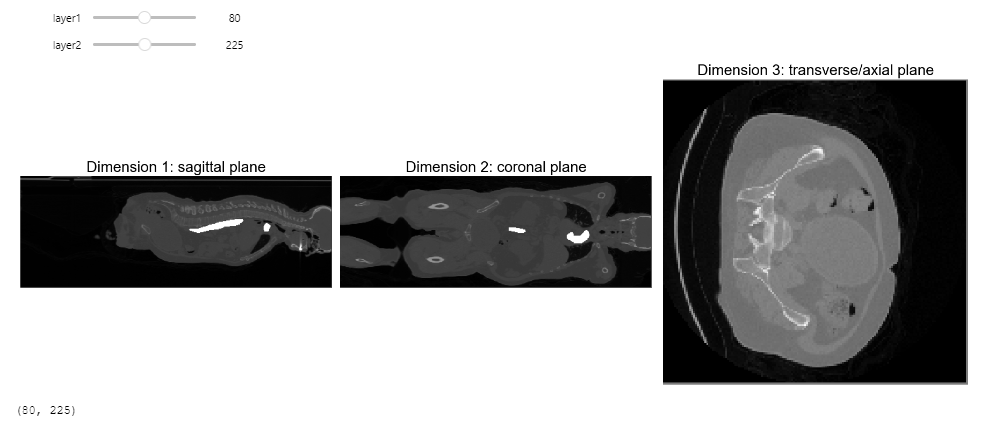
\includegraphics{images/slider5.PNG}
\caption{Slider5}
\end{figure}

    We can clearly see the typical shape of the aorta, including the
transverse arch and ascending and descending thoracic.

    \hypertarget{task-2}{%
\subsection{Task 2}\label{task-2}}

    \hypertarget{calculate-the-volume-of-the-segmented-aorta-in-segmentation.nii.gz-in-millilitres}{%
\subsubsection{\texorpdfstring{Calculate the volume of the segmented
aorta (in \texttt{segmentation.nii.gz}) in
\textbf{millilitres}}{Calculate the volume of the segmented aorta (in segmentation.nii.gz) in millilitres}}\label{calculate-the-volume-of-the-segmented-aorta-in-segmentation.nii.gz-in-millilitres}}

    \begin{tcolorbox}[breakable, size=fbox, boxrule=1pt, pad at break*=1mm,colback=cellbackground, colframe=cellborder]
\prompt{In}{incolor}{12}{\boxspacing}
\begin{Verbatim}[commandchars=\\\{\}]
\PY{n}{flat} \PY{o}{=} \PY{n}{seg\PYZus{}mtx}\PY{o}{.}\PY{n}{flatten}\PY{p}{(}\PY{p}{)}   
\PY{n+nb}{set}\PY{p}{(}\PY{n}{flat}\PY{p}{)}
\end{Verbatim}
\end{tcolorbox}

            \begin{tcolorbox}[breakable, size=fbox, boxrule=.5pt, pad at break*=1mm, opacityfill=0]
\prompt{Out}{outcolor}{12}{\boxspacing}
\begin{Verbatim}[commandchars=\\\{\}]
\{0.0, 1.0\}
\end{Verbatim}
\end{tcolorbox}
        
    We thereby see, that the voxels are represented by binary values
\texttt{\{0:\ \textquotesingle{}black\textquotesingle{},\ 1:\ \textquotesingle{}white\textquotesingle{}\}}.\textbackslash{}

Thereby, to compute the volume of the aorta artery, we just need to
count the number of voxels, compute the volume of a voxel, and perform
simple calculus.\textbackslash{}

Note, that \(1,000,000\;mm^3 = 1\;liter = 1\;dm^3\) \textbackslash{}

The calculation to determine the volume of the aorta can be done in
various ways. Here are two of them:

    \begin{tcolorbox}[breakable, size=fbox, boxrule=1pt, pad at break*=1mm,colback=cellbackground, colframe=cellborder]
\prompt{In}{incolor}{13}{\boxspacing}
\begin{Verbatim}[commandchars=\\\{\}]
\PY{n+nb}{print}\PY{p}{(}\PY{l+s+s2}{\PYZdq{}}\PY{l+s+s2}{Volume computed with original (anisotropic) image:}\PY{l+s+se}{\PYZbs{}n}\PY{l+s+s2}{\PYZdq{}}\PY{p}{)}
\PY{n}{white\PYZus{}voxels} \PY{o}{=} \PY{n}{np}\PY{o}{.}\PY{n}{sum}\PY{p}{(}\PY{n}{seg\PYZus{}mtx} \PY{o}{==} \PY{l+m+mi}{1}\PY{p}{)}  

\PY{n+nb}{print}\PY{p}{(}\PY{l+s+s2}{\PYZdq{}}\PY{l+s+s2}{approach 1:}\PY{l+s+s2}{\PYZdq{}}\PY{p}{)}
\PY{n}{volume} \PY{o}{=} \PY{n}{np}\PY{o}{.}\PY{n}{sum}\PY{p}{(}\PY{n}{seg\PYZus{}mtx}\PY{p}{)} \PY{o}{*} \PY{n}{np}\PY{o}{.}\PY{n}{prod}\PY{p}{(}\PY{n}{seg\PYZus{}img}\PY{o}{.}\PY{n}{header}\PY{o}{.}\PY{n}{get\PYZus{}zooms}\PY{p}{(}\PY{p}{)}\PY{p}{)} \PY{o}{/} \PY{l+m+mi}{1000\PYZus{}000} \PY{c+c1}{\PYZsh{} convert to litres}
\PY{n+nb}{print}\PY{p}{(}\PY{l+s+sa}{f}\PY{l+s+s1}{\PYZsq{}}\PY{l+s+s1}{The volume of the segmented aorta is }\PY{l+s+si}{\PYZob{}}\PY{n}{volume}\PY{+w}{ }\PY{o}{*}\PY{+w}{ }\PY{l+m+mi}{1000}\PY{l+s+si}{\PYZcb{}}\PY{l+s+s1}{ millilitres.}\PY{l+s+se}{\PYZbs{}n}\PY{l+s+s1}{\PYZsq{}}\PY{p}{)} \PY{c+c1}{\PYZsh{} convert to millilitres}

\PY{n+nb}{print}\PY{p}{(}\PY{l+s+s2}{\PYZdq{}}\PY{l+s+s2}{approach 2:}\PY{l+s+s2}{\PYZdq{}}\PY{p}{)}
\PY{c+c1}{\PYZsh{} to get the volume, we need to consider the voxel sizes (x*y*z)}
\PY{n}{voxel\PYZus{}vol} \PY{o}{=} \PY{n}{seg\PYZus{}img}\PY{o}{.}\PY{n}{header}\PY{o}{.}\PY{n}{get\PYZus{}zooms}\PY{p}{(}\PY{p}{)}\PY{p}{[}\PY{l+m+mi}{0}\PY{p}{]} \PY{o}{*} \PY{n}{seg\PYZus{}img}\PY{o}{.}\PY{n}{header}\PY{o}{.}\PY{n}{get\PYZus{}zooms}\PY{p}{(}\PY{p}{)}\PY{p}{[}\PY{l+m+mi}{1}\PY{p}{]} \PY{o}{*} \PY{n}{seg\PYZus{}img}\PY{o}{.}\PY{n}{header}\PY{o}{.}\PY{n}{get\PYZus{}zooms}\PY{p}{(}\PY{p}{)}\PY{p}{[}\PY{l+m+mi}{2}\PY{p}{]}   
\PY{n}{white\PYZus{}voxel\PYZus{}vol} \PY{o}{=} \PY{n}{white\PYZus{}voxels} \PY{o}{*} \PY{n}{voxel\PYZus{}vol}

\PY{n+nb}{print}\PY{p}{(}\PY{l+s+s2}{\PYZdq{}}\PY{l+s+s2}{Volume of Aorta:}\PY{l+s+s2}{\PYZdq{}}\PY{p}{,} \PY{n}{white\PYZus{}voxel\PYZus{}vol}\PY{p}{,} \PY{l+s+s2}{\PYZdq{}}\PY{l+s+s2}{cubic milimeters}\PY{l+s+s2}{\PYZdq{}}\PY{p}{)}
\PY{n+nb}{print}\PY{p}{(}\PY{l+s+s2}{\PYZdq{}}\PY{l+s+s2}{Volume of Aorta:}\PY{l+s+s2}{\PYZdq{}}\PY{p}{,} \PY{n}{white\PYZus{}voxel\PYZus{}vol}\PY{o}{/}\PY{l+m+mi}{10}\PY{o}{*}\PY{o}{*}\PY{p}{(}\PY{l+m+mi}{3}\PY{o}{+}\PY{l+m+mi}{3}\PY{p}{)} \PY{o}{*} \PY{l+m+mi}{1000}\PY{p}{,} \PY{l+s+s2}{\PYZdq{}}\PY{l+s+s2}{millilitres}\PY{l+s+s2}{\PYZdq{}}\PY{p}{)}
\PY{n+nb}{print}\PY{p}{(}\PY{l+s+s2}{\PYZdq{}}\PY{l+s+s2}{Volume of Aorta:}\PY{l+s+s2}{\PYZdq{}}\PY{p}{,} \PY{n}{white\PYZus{}voxel\PYZus{}vol}\PY{o}{/}\PY{l+m+mi}{10}\PY{o}{*}\PY{o}{*}\PY{p}{(}\PY{l+m+mi}{3}\PY{o}{+}\PY{l+m+mi}{3}\PY{p}{)}\PY{p}{,} \PY{l+s+s2}{\PYZdq{}}\PY{l+s+s2}{litres}\PY{l+s+s2}{\PYZdq{}}\PY{p}{)}
\end{Verbatim}
\end{tcolorbox}

    \begin{Verbatim}[commandchars=\\\{\}]
Volume computed with original (anisotropic) image:

approach 1:
The volume of the segmented aorta is 323.7954567146301 millilitres.

approach 2:
Volume of Aorta: 323795.4567146301 cubic milimeters
Volume of Aorta: 323.7954567146301 millilitres
Volume of Aorta: 0.3237954567146301 litres
    \end{Verbatim}

    \begin{tcolorbox}[breakable, size=fbox, boxrule=1pt, pad at break*=1mm,colback=cellbackground, colframe=cellborder]
\prompt{In}{incolor}{14}{\boxspacing}
\begin{Verbatim}[commandchars=\\\{\}]
\PY{n+nb}{print}\PY{p}{(}\PY{l+s+s2}{\PYZdq{}}\PY{l+s+s2}{Volume computed with resampled (isotropic) image:}\PY{l+s+se}{\PYZbs{}n}\PY{l+s+s2}{\PYZdq{}}\PY{p}{)}
\PY{n}{white\PYZus{}voxels} \PY{o}{=} \PY{n}{np}\PY{o}{.}\PY{n}{sum}\PY{p}{(}\PY{n}{resampled\PYZus{}seg\PYZus{}mtx} \PY{o}{==} \PY{l+m+mi}{1}\PY{p}{)}  

\PY{n+nb}{print}\PY{p}{(}\PY{l+s+s2}{\PYZdq{}}\PY{l+s+s2}{approach 1:}\PY{l+s+s2}{\PYZdq{}}\PY{p}{)}
\PY{n}{volume} \PY{o}{=} \PY{n}{np}\PY{o}{.}\PY{n}{sum}\PY{p}{(}\PY{n}{resampled\PYZus{}seg\PYZus{}mtx}\PY{p}{)} \PY{o}{*} \PY{n}{np}\PY{o}{.}\PY{n}{prod}\PY{p}{(}\PY{n}{resampled\PYZus{}seg\PYZus{}img}\PY{o}{.}\PY{n}{header}\PY{o}{.}\PY{n}{get\PYZus{}zooms}\PY{p}{(}\PY{p}{)}\PY{p}{)} \PY{o}{/} \PY{l+m+mi}{1000\PYZus{}000} 
\PY{n+nb}{print}\PY{p}{(}\PY{l+s+sa}{f}\PY{l+s+s1}{\PYZsq{}}\PY{l+s+s1}{The volume of the segmented aorta is }\PY{l+s+si}{\PYZob{}}\PY{n}{volume}\PY{o}{*}\PY{l+m+mi}{1000}\PY{l+s+si}{\PYZcb{}}\PY{l+s+s1}{ millilitres.}\PY{l+s+se}{\PYZbs{}n}\PY{l+s+s1}{\PYZsq{}}\PY{p}{)} 

\PY{n+nb}{print}\PY{p}{(}\PY{l+s+s2}{\PYZdq{}}\PY{l+s+s2}{approach 2:}\PY{l+s+s2}{\PYZdq{}}\PY{p}{)}
\PY{n}{voxel\PYZus{}vol} \PY{o}{=} \PY{n}{resampled\PYZus{}seg\PYZus{}img}\PY{o}{.}\PY{n}{header}\PY{o}{.}\PY{n}{get\PYZus{}zooms}\PY{p}{(}\PY{p}{)}\PY{p}{[}\PY{l+m+mi}{0}\PY{p}{]} \PY{o}{*} \PY{n}{resampled\PYZus{}seg\PYZus{}img}\PY{o}{.}\PY{n}{header}\PY{o}{.}\PY{n}{get\PYZus{}zooms}\PY{p}{(}\PY{p}{)}\PY{p}{[}\PY{l+m+mi}{1}\PY{p}{]} \PY{o}{*} \PY{n}{resampled\PYZus{}seg\PYZus{}img}\PY{o}{.}\PY{n}{header}\PY{o}{.}\PY{n}{get\PYZus{}zooms}\PY{p}{(}\PY{p}{)}\PY{p}{[}\PY{l+m+mi}{2}\PY{p}{]}   
\PY{n}{white\PYZus{}voxel\PYZus{}vol} \PY{o}{=} \PY{n}{white\PYZus{}voxels} \PY{o}{*} \PY{n}{voxel\PYZus{}vol}

\PY{n+nb}{print}\PY{p}{(}\PY{l+s+s2}{\PYZdq{}}\PY{l+s+s2}{Volume of Aorta:}\PY{l+s+s2}{\PYZdq{}}\PY{p}{,} \PY{n}{white\PYZus{}voxel\PYZus{}vol}\PY{p}{,} \PY{l+s+s2}{\PYZdq{}}\PY{l+s+s2}{cubic milimeters}\PY{l+s+s2}{\PYZdq{}}\PY{p}{)}
\PY{n+nb}{print}\PY{p}{(}\PY{l+s+s2}{\PYZdq{}}\PY{l+s+s2}{Volume of Aorta:}\PY{l+s+s2}{\PYZdq{}}\PY{p}{,} \PY{n}{white\PYZus{}voxel\PYZus{}vol}\PY{o}{/}\PY{l+m+mi}{10}\PY{o}{*}\PY{o}{*}\PY{p}{(}\PY{l+m+mi}{3}\PY{o}{+}\PY{l+m+mi}{3}\PY{p}{)} \PY{o}{*} \PY{l+m+mi}{1000}\PY{p}{,} \PY{l+s+s2}{\PYZdq{}}\PY{l+s+s2}{millilitres}\PY{l+s+s2}{\PYZdq{}}\PY{p}{)}
\PY{n+nb}{print}\PY{p}{(}\PY{l+s+s2}{\PYZdq{}}\PY{l+s+s2}{Volume of Aorta:}\PY{l+s+s2}{\PYZdq{}}\PY{p}{,} \PY{n}{white\PYZus{}voxel\PYZus{}vol}\PY{o}{/}\PY{l+m+mi}{10}\PY{o}{*}\PY{o}{*}\PY{p}{(}\PY{l+m+mi}{3}\PY{o}{+}\PY{l+m+mi}{3}\PY{p}{)}\PY{p}{,} \PY{l+s+s2}{\PYZdq{}}\PY{l+s+s2}{litres}\PY{l+s+s2}{\PYZdq{}}\PY{p}{)}
\end{Verbatim}
\end{tcolorbox}

    \begin{Verbatim}[commandchars=\\\{\}]
Volume computed with resampled (isotropic) image:

approach 1:
The volume of the segmented aorta is 325.10699999999997 millilitres.

approach 2:
Volume of Aorta: 325107.0 cubic milimeters
Volume of Aorta: 325.10699999999997 millilitres
Volume of Aorta: 0.325107 litres
    \end{Verbatim}

    The volume of the isotropic and anisotropic sligthly differ by
\(\approx\) 1.3 millilitres. This may be due to the interpolation that
is necessary to resample the image.

    \begin{tcolorbox}[breakable, size=fbox, boxrule=1pt, pad at break*=1mm,colback=cellbackground, colframe=cellborder]
\prompt{In}{incolor}{18}{\boxspacing}
\begin{Verbatim}[commandchars=\\\{\}]
\PY{o}{!}jupyter\PY{+w}{ }nbconvert\PY{+w}{ }\PYZhy{}\PYZhy{}to\PY{+w}{ }latex\PY{+w}{ }development.ipynb
\end{Verbatim}
\end{tcolorbox}

    \begin{Verbatim}[commandchars=\\\{\}]
[NbConvertApp] Converting notebook development.ipynb to latex
C:\textbackslash{}Users\textbackslash{}marku\textbackslash{}miniconda3\textbackslash{}Lib\textbackslash{}site-packages\textbackslash{}nbconvert\textbackslash{}utils\textbackslash{}pandoc.py:51:
RuntimeWarning: You are using an unsupported version of pandoc (2.12).
Your version must be at least (2.14.2) but less than (4.0.0).
Refer to https://pandoc.org/installing.html.
Continuing with doubts{\ldots}
  check\_pandoc\_version()
[NbConvertApp] Support files will be in development\_files\textbackslash{}
[NbConvertApp] Making directory development\_files
[NbConvertApp] Writing 78154 bytes to development.tex
    \end{Verbatim}

    \begin{tcolorbox}[breakable, size=fbox, boxrule=1pt, pad at break*=1mm,colback=cellbackground, colframe=cellborder]
\prompt{In}{incolor}{20}{\boxspacing}
\begin{Verbatim}[commandchars=\\\{\}]
\PY{o}{!}jupyter\PY{+w}{ }nbconvert\PY{+w}{ }\PYZhy{}\PYZhy{}to\PY{+w}{ }markdown\PY{+w}{ }development.ipynb\PY{+w}{ }\PYZhy{}\PYZhy{}output\PY{+w}{ }README.md
\end{Verbatim}
\end{tcolorbox}

    \begin{Verbatim}[commandchars=\\\{\}]
[NbConvertApp] Converting notebook development.ipynb to markdown
[NbConvertApp] Support files will be in README\_files\textbackslash{}
[NbConvertApp] Making directory README\_files
[NbConvertApp] Writing 20263 bytes to README.md
    \end{Verbatim}


    % Add a bibliography block to the postdoc
    
    
    
\end{document}
